% !TEX encoding = UTF-8
% !TEX TS-program = pdflatex
% !TEX root = ../tesi.tex

%**************************************************************
\chapter{Progettazione e codifica}
\label{cap:progettazione-codifica}
%**************************************************************

\intro{Il seguente capitolo descrive gli strumenti e la progettazione con cui
    sono
    state implementate le integrazione con la \textit{web app} \productName.}\\

%**************************************************************
\section{Tecnologie}
\label{sec:tecnologie-strumenti}

Di seguito viene data una panoramica delle tecnologie e strumenti utilizzati.

\subsection*{Java}
Java è un linguaggio di programmazione e una piattaforma di elaborazione
rilasciato per la prima volta da Sun Microsystems nel 1995. Si è evoluto da
umili
origini per sostenere gran parte del mondo digitale di oggi, fornendo una
piattaforma affidabile su cui sono costruiti molti servizi e applicazioni.
Anche i nuovi prodotti, innovativi nei servizi digitali progettati per il
futuro,
continuano a fare affidamento su Java. \cite{site-what-is-java} \\
\subsection*{Spring}

Spring è un \gls{framework} open source per lo sviluppo di applicazioni su
piattaforma Java.
A questo \gls{framework} sono associati tanti altri progetti, che hanno nomi
composti come
Spring Boot, Spring Data, Spring Batch, etc. Questi progetti sono stati ideati
per
fornire funzionalità aggiuntive al \gls{framework}. \cite{site-spring}

\subsection*{Typescript}
%**************************************************************
TypeScript è un linguaggio di programmazione sviluppato e gestito da Microsoft.

\noindent È un \gls{superset} di JavaScript, permettendo di aggiungere la
tipizzazione
statica opzionale al linguaggio. TypeScript è progettato per lo sviluppo di
applicazioni
di grandi dimensioni e per la \gls{transcompilazione} in JavaScript. Poiché
TypeScript è un \gls{superset} di JavaScript, anche i programmi JavaScript
esistenti sono validi programmi TypeScript. \cite{site-typescript}
\subsection*{Angular}
%**************************************************************
Angular è un \gls{framework} JavaScript per applicazioni \textit{web}
dinamiche, utilizzato in particolare per la creazione di \gls{spa} e
\textit{web app}. Consente di utilizzare HTML come linguaggio \textit{template}
e di estenderne la sintassi per esprimere le componenti di un'applicazione in
modo chiaro e succinto.
% TODO: aggiungere bibliografia, link: https://psicografici.com/angular-js/#:~:text=Angular%20%C3%A8%20un%20framework%20JavaScript,in%20modo%20chiaro%20e%20succinto.

\subsection*{Angular Material}
%**************************************************************
Angular Material è una libreria sviluppata da Google nel 2014 progettata per
aiutare a sviluppare pagine \textit{web} in modo strutturato. \\
I suoi componenti aiutano a creare pagine \textit{web} e applicazioni
\textit{web} attraenti, coerenti e funzionali. \cite{site-Angular}

\subsection*{Node.js}
Node.js è una piattaforma di sviluppo open source per l'esecuzione di codice
JavaScript lato \textit{server}. Node è utile per sviluppare applicazioni che
richiedono una connessione permanente dal \textit{browser} al \textit{server}
ed è spesso utilizzato per applicazioni in tempo reale come chat, feed di
notizie e di notifiche.\\
Node.js è utilizzato da Angular per gestire le dipendenze, permettendo la
dichiarazione di due insiemi di dipendenze: per gli sviluppatori e per far
funzionare l'applicativo. In questo modo è possibile differenziare quali
librerie si possono tralasciare in fase di \textit{deploy} dell'applicazione
perché, ad esempio, necessarie solo per effettuare i test. \cite{site-node}
%**************************************************************
\section{Progettazione}
\label{sec:progettazione}

\subsection{Back end}
\subsubsection{Architettura Spring Boot}
Spring Boot è un modulo di Spring \gls{framework}. Viene utilizzato per creare
applicazioni \textit{stand-alone} di livello produttivo con il minimo sforzo.\\
Spring Boot segue un'architettura a strati, in cui ogni livello comunica con
gli strati vicini.\\
Ci sono quattro strati in Spring Boot, che sono i seguenti:
\begin{itemize}
    \item \textbf{\textit{Presentation layer}:} gestisce le richieste HTTP,
          trasforma i parametri da formato JSON in classe e autentica la
          richiesta, per
          poi trasferirla al \textit{business layer};
    \item \textbf{\textit{Business Layer}:} gestisce tutta la \textit{business
              logic}. Consiste in classi di servizio e utilizza servizi forniti
          dagli strati
          di accesso ai dati;
    \item \textbf{\textit{Persistence Layer}:} contiene tutta la
          \textit{storage logic}, e trasformando gli oggetti provenienti dalla
          \textit{business logic} in righe del \textit{database};
    \item \textbf{\textit{Database Layer}:} in questo strato vengono effettuate
          le operazioni \gls{CRUD}.
\end{itemize}
\begin{figure}[H]
    \centering
    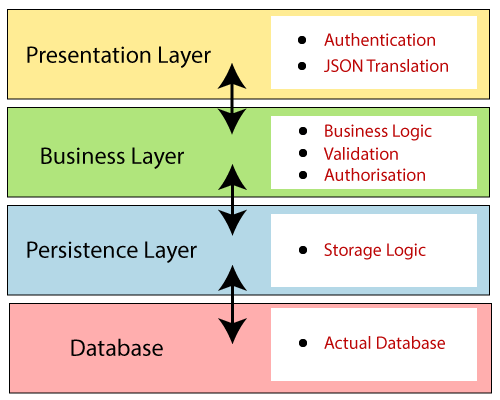
\includegraphics[scale=0.3]{spring-boot-architecture-layer.png}
    \caption{Architettura a strati di Spring Boot}
\end{figure}

\subsubsection{Spring Boot Flow Architecture}
\begin{figure}[H]
    \centering
    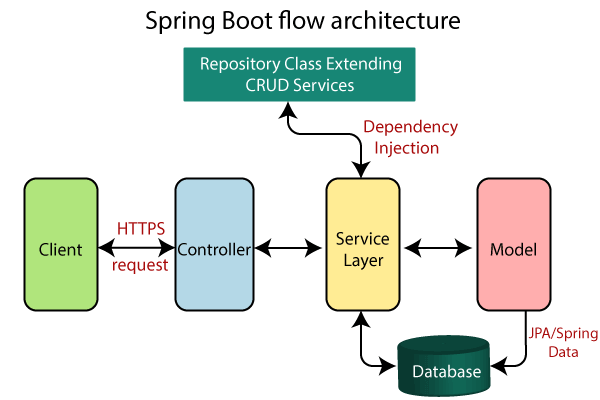
\includegraphics[width=1\columnwidth]{spring-boot-architecture.png}
    \caption{Spring Boot \textit{workflow}}
\end{figure}
Il \textit{workflow} con cui vengono effettuate richieste HTTP utilizzando
Spring Boot è il seguente:
\begin{itemize}
    \item il \textit{client} esegue una richiesta HTTP (GET, POST, PUT O DELETE) ad un
          \gls{endpoint} esposto;
    \item la richiesta viene ricevuta dal \textit{controller}, che mappa la
          richiesta e la gestisce. Dopodiché chiama la \textit{service logic}
          presente
          nel \textit{service layer};
    \item nel \textit{service layer} viene eseguita la \textit{business logic}.
          Vengono eseguite le operazioni sulle classi mappate nel
          \textit{database};
    \item il \textit{repository} \textit{JpaRepository} esegue le operazioni
          sul \textit{database};
    \item una pagina \gls{JSP} viene restituita all'utente se non si è
          verificato un errore. \cite{site-microservizi}
\end{itemize}

\subsubsection{Progettazione delle API}
Il \textit{back end} del progetto è strutturato a \glspl{microservizio}, ognuno
contenente una \textit{business logic} atta a soddisfare un certo tipo di
richieste.\\
Il \textit{front end} comunica con il \textit{back end} attraverso gli
\gls{endpoint} che ogni \gls{microservizio} espone. \\
Tuttavia, effettuare connessioni dirette fra \textit{front end} e ogni
\gls{microservizio} presenta alcuni problemi, come:
\begin{itemize}
    \item numerose connessioni a seconda della quantità dei
          \glspl{microservizio};
    \item i \glspl{microservizio} devono esporre pubblicamente il proprio
          \gls{IP}, causando problemi sia di sicurezza, dovuta all'esposizione
          degli
          indirizzi \gls{IP} al mondo esterno, sia in fase di latenza, ovvero
          il tempo
          che intercorre tra l'invio di una richiesta ed una risposta tenderà
          ad essere
          sempre più alto. \cite{site-api-gateway}
\end{itemize}

\noindent Per far fronte a queste problematiche si è deciso di utilizzare un
\nameref{sub:ApiGateway}.\\
In questo modo, solamente un \gls{IP} sarà visibile pubblicamente, mentre
quelli dei \glspl{microservizio} possono diventare privati.\\
Per quanto riguarda la latenza, il \textit{front end} comunicherà attraverso
l'\nameref{sub:ApiGateway}, stabilendo solo le connessioni per la richiesta e
la risposta, lasciando all'\nameref{sub:ApiGateway} il compito di smistare le
richieste al giusto \gls{microservizio}, rendendo così la connessione più
rapida rispetto all'utilizzo di diverse connessioni per ogni
\gls{microservizio}, essendo tutte le richieste effettuate all'interno dello
stesso \textit{network}.

\subsection{Front end}
\subsubsection{Architettura Angular}
Il componente principale di Angular è il \textbf{modulo}. Un modulo è un
contenitore di funzionalità che sono esposte ad altri moduli. Questa
suddivisione in moduli rende la struttura dell'applicazione ordinata e il
codice mantenibile.\\
Un elemento fondamentale di Angular è il \class{component}, ovvero delle classi
che gestiscono le \textit{view} dell'applicazione e la loro logica.\\
I dati da visualizzare nella \textit{view} vengono forniti dalle classi dette
\textbf{servizi}. Queste classi svolgono diverse funzioni, come per esempio
l'esecuzione delle richieste HTTP.\\
Ad ogni component è associato un \textit{template}, ovvero del codice HTML in
cui si definisce come viene visualizzato il \textit{component}.\\
È possibile personalizzare il codice HTML utilizzando le \textbf{direttive},
ovvero delle classi che aggiungono un comportamento aggiuntivo agli elementi
nelle applicazioni Angular. Le direttive integrate di Angular permettono di
gestire moduli, elenchi, stili e ciò che gli utenti vedono.\\
È possibile creare un \textit{component} che rappresenta la pagina completa, in
cui inserire diversi \textit{component} per ogni elemento contenuto in quella
pagina.
Ogni \textit{component} contenuto si occuperà così di gestire la grafica di
quella determinata funzionalità e di comunicare con i servizi di cui necessita;
sarà poi il \textit{component} \enquote*{padre} a gestire la disposizione dei
\textit{component} utilizzati. \cite{site-angular-concepts}

\subsubsection{Progettazione delle maschere}
Con il \textit{tutor} aziendale è stato discusso come dovrebbero essere
graficamente le nuove maschere da aggiungere a \productName. A partire da
questi confronti, è stato poi utilizzato \textbf{Figma} per fare il
\textit{mockup}, in modo da  testare quanto siano accattivanti i vari elementi visivi.\\
Durante la progettazione del \textit{mockup} è stato seguito lo stile presente
nella \textit{web app}, in modo da non disorientare l'utente durante la
navigazione. \\
I risultati della progettazione delle maschere sono riportati in seguito.
\begin{figure}[H]
    \centerline{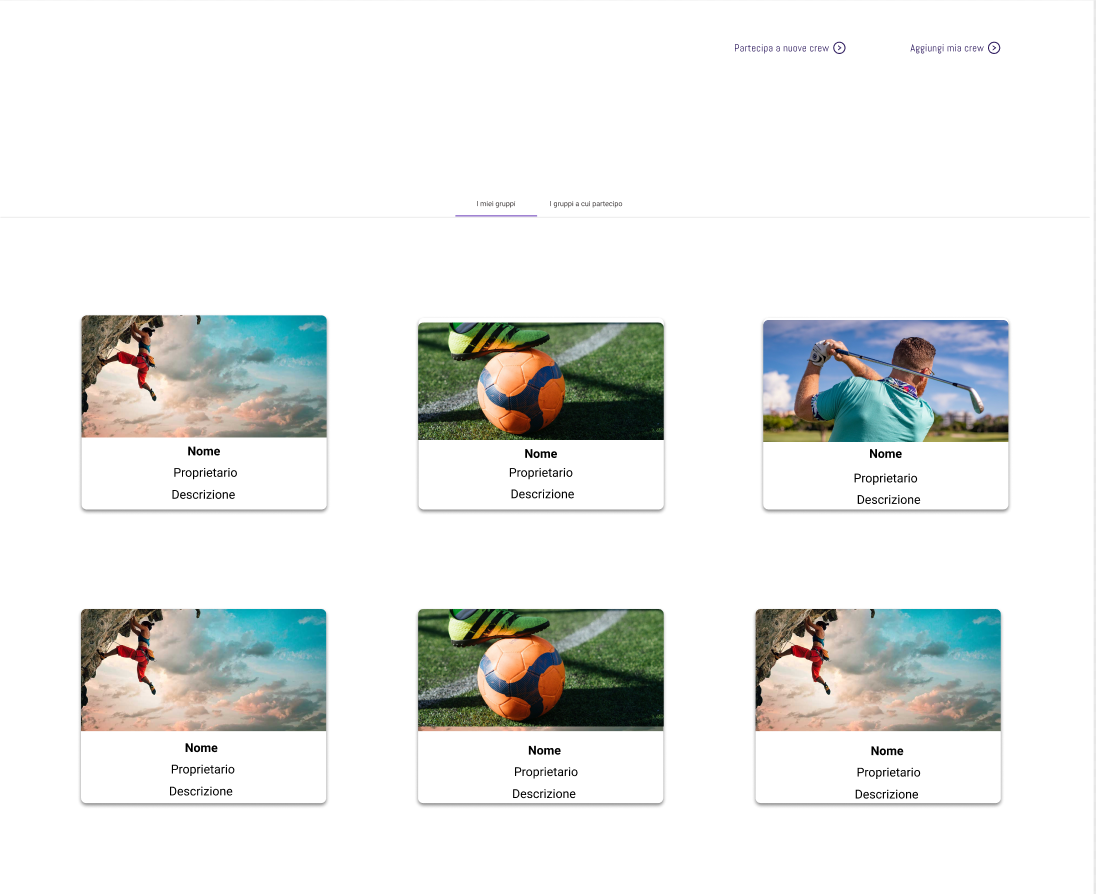
\includegraphics[scale=0.9]{mockup/le-mie-crew.png}}
    \caption{\textit{Mockup} pagina per la visualizzazione dei gruppi creati
        dall'utente}
\end{figure}

% \begin{figure}[H] 
%     \centering 
%     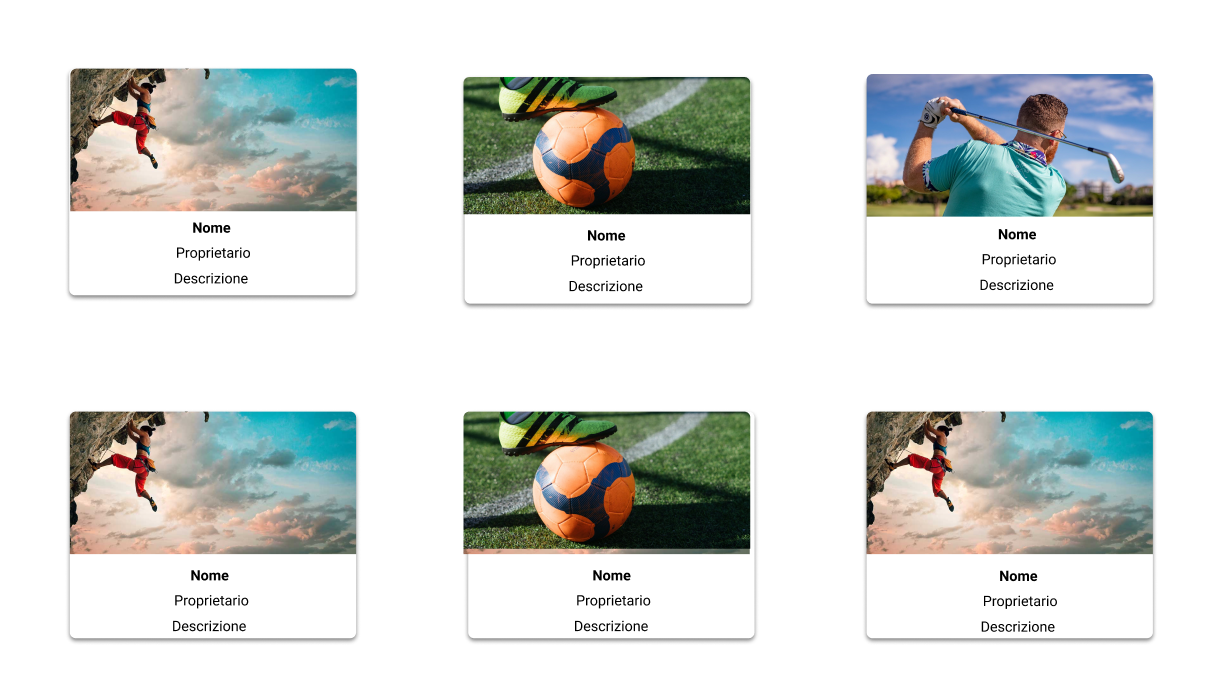
\includegraphics[scale=0.6]{mockup/lista-crew.png} 
%     \caption{\textit{Mockup} pagina per la visualizzazione dei gruppi a cui partecipa l'utente}
% \end{figure}

\begin{figure}[H]
    \centering
    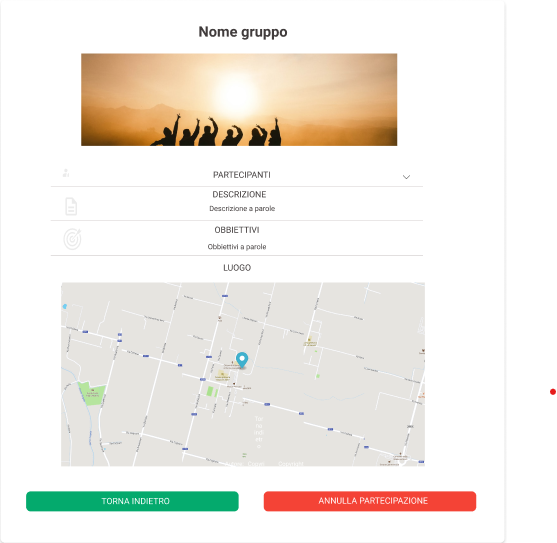
\includegraphics[scale=0.8]{mockup/dettagli-crew.png}
    \caption{\textit{Mockup} pagina per la visualizzazione dei dettagli di un
        gruppo}
\end{figure}

\begin{figure}[H]
    \centering
    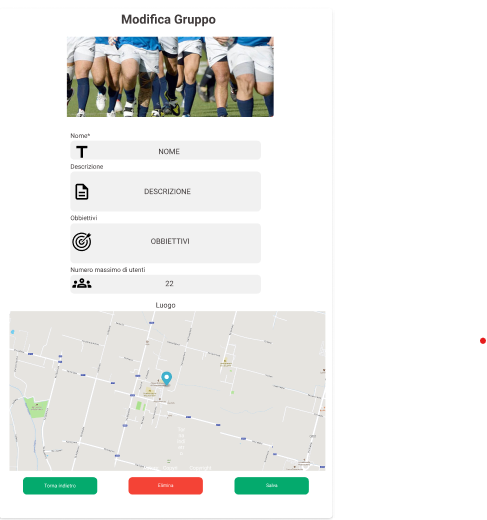
\includegraphics[scale=0.8]{mockup/modifica-crew.png}
    \caption{\textit{Mockup} pagina per la modifica dei dettagli di un gruppo}
\end{figure}

Come si può notare dalle immagini, sono stati omessi dalla progettazione
l'\textit{header} e il \textit{footer}, in quanto sono già presenti nella
\textit{web app}.

% \subsubsection{Namespace 1} %**************************
% Descrizione namespace 1.

% \begin{namespacedesc}
%     \classdesc{Classe 1}{Descrizione classe 1}
%     \classdesc{Classe 2}{Descrizione classe 2}
% \end{namespacedesc}

%**************************************************************
\section{Design Pattern utilizzati}
\subsection{Microservizi}
I \glspl{microservizio} sono un approccio per lo sviluppo e l'organizzazione
dell'architettura \textit{software} secondo cui quest'ultimi sono composti di
servizi indipendenti di piccole dimensioni che comunicano tra loro tramite
\gls{API} ben definite.\\
Nel contesto di questo progetto, sono stati implementati tre
\glspl{microservizio}:
\begin{itemize}
    \item \textbf{SW\_Gruppi}: \gls{microservizio} responsabile per la gestione
          delle funzionalità legate ai gruppi;
    \item \textbf{ApiGateway}: \gls{microservizio} che implementa il
          \textit{pattern} \nameref{sub:ApiGateway};
    \item \textbf{EurekaServer}: \gls{microservizio} che implementa il pattern
          \hyperref[sub:ServiceRegistry]{ServiceRegistry}.
          \cite{site-microservizi-aws}
\end{itemize}
\subsection{API Gateway}
\label{sub:ApiGateway}
\begin{figure}[H]
    \centering
    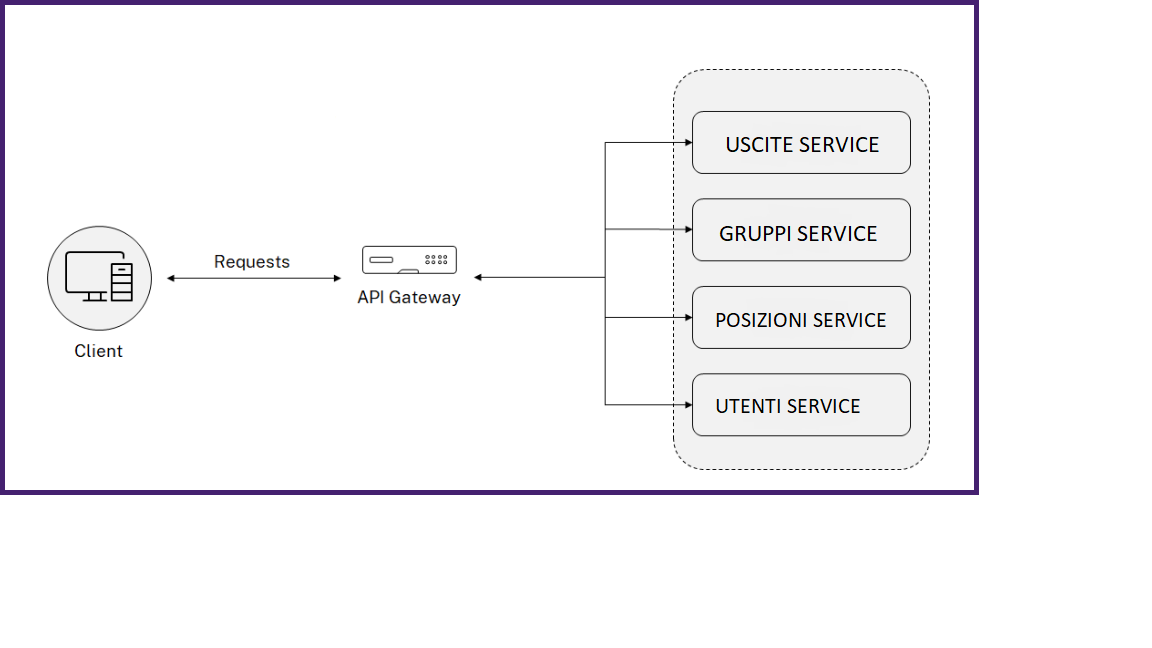
\includegraphics[scale=0.68]{progettazione/API-Gateway.png}
    \caption{Diagramma concettuale che descrive l'\textit{API Gateway}}
\end{figure}
Un \class{API Gateway} è uno strumento di gestione delle \gls{API} che si situa
tra un \textit{client} e una raccolta di servizi \textit{back end}. Un
\textit{API Gateway} si comporta come un \textit{proxy} inverso per riceve
tutte le chiamate \gls{API}, aggregando le chiamate alle \gls{API} dei servizi
richiesti, gestendo e restituendo i risultati appropriati in base alle
richieste ricevute.\\
Utilizzare un \textit{API Gateway} è vantaggioso perché:
\begin{itemize}
    \item permette di centralizzare il punto di ingresso per le chiamate;
    \item permette di monitorare le risorse utilizzate;
    \item permette di proteggere un servizio che è aperto a tutti;
    \item ha latenza minore rispetto alla chiamata a diversi servizi.
\end{itemize}

\subsection{Client-Side Service Discovery e Service Registry}
\label{sub:ServiceRegistry}
\begin{figure}[H]
    \centering
    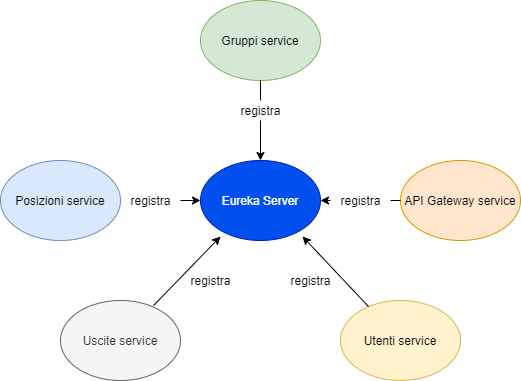
\includegraphics[scale=0.4]{progettazione/registrazione-servizi.png}
    \caption{Diagramma concettuale che descrive la registrazione dei
        microservizi all'\gls{Eureka Server}}
\end{figure}
% TODO: aggungere bibliografia: https://lalverma.medium.com/spring-boot-microservices-implementing-service-discovery-cfc98e49b74f, https://microservices.io/patterns/service-registry.html
I \glspl{microservizio} hanno una natura dinamica, in quanto è possibile che
più istanze di un singolo \gls{microservizio} coesistano, probabilmente
esponendo le loro \gls{API} in un indirizzo \gls{IP} diverso o in una porta
diversa. Queste evenienze portano all'impossibilità di:
\begin{itemize}
    \item conoscere la posizione di qualsiasi istanza dei
          \glspl{microservizio};
    \item tenere traccia di tutte le istanze;
    \item selezionare un'istanza di \gls{microservizio}.
\end{itemize}
La soluzione a questi problemi è l'utilizzo del \textit{pattern}
\textbf{\textit{Client-side Service Discovery}}, che fornisce un meccanismo che
tiene traccia di tutti i servizi e delle relative istanze. Tutti i
\glspl{microservizio} si registrano ad un \textit{Service registry} e
continuano ad aggiornare regolarmente le proprie informazioni di
rete.\cite{site-spring-boot-microservizi}\\
Il \textit{pattern} \textbf{\textit{Service registry}} è stato applicato
mediante l'implementazione di un \class{Eureka Server}. L'\textit{Eureka
    Server} è un \textit{database} di servizi che tiene traccia di ogni
\gls{microservizio}, delle loro istanze e delle loro locazioni. I
\glspl{microservizio} si registrano all'avvio dell'applicazione e vengono
rimossi alla sua chiusura.\\
L'utilizzo di questi \textit{pattern}  permette ai servizi di comunicare fra di
loro, ottenendo le informazioni degli altri servizi direttamente
dall'\gls{Eureka Server}.\cite{site-service-registry}
\subsection{Dependency Injection}
\label{sub:Dependency-Injection}
Sia Angular sia Spring sono dei \gls{framework} che implementano delle
convenzioni che permettono l'utilizzo del \textit{pattern} \class{Dependency
    Injection}.\\
L'ecosistema all'interno del quale le applicazioni Spring vivono viene definito
\class{IoC container}. L'\textit{IoC container} si occupa di istanziare gli
oggetti (\textit{beans}) dichiarati nel progetto e di reperire e iniettare
tutte le dipendenze ad essi associate. Tali dipendenze possono essere
componenti del \gls{framework} o altri \textit{bean} dichiarati nel contesto
applicativo.\\
La dichiarazione di una classe come componente nel progetto avviene tramite
l'utilizzo dell'annotazione \code{@Component}, che rappresenta la categoria più
generica per la dichiarazione di un componente.
Durante la fase di codifica del progetto sono state utilizzate le annotazioni
\code{@RestController}, \code{@Service} e \code{@Repository}, che sono delle
specializzazioni dell'annotazione \code{@Component}.\\
Per iniettare delle classi da recuperare dal \textit{IoC container} è
sufficiente utilizzare l'annotazione
\code{@Autowired}.\cite{site-dependency-injection-spring}
% \begin{figure}[H] 
%     \centering 
%     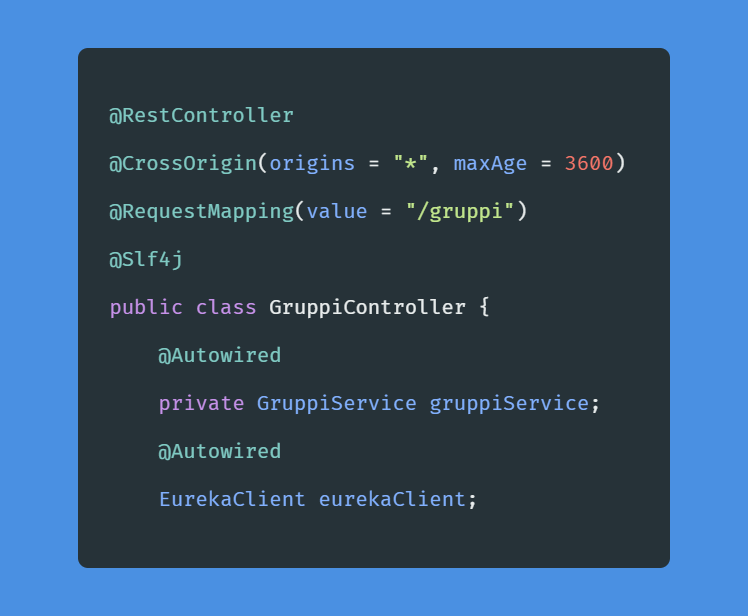
\includegraphics[scale=0.2]{progettazione/autowired-code.png}
%     \caption{Esempio di \textit{Dependency Injection} con Spring}
% \end{figure}

\begin{lstlisting}[style = Java, caption = {Esempio di \textit{Dependency Injection} con Spring}]
@RestController
@CrossOrigin(origins = "*", maxAge = 3600)
@RequestMapping(value = "/gruppi")
public class GruppiController {

    @Autowired
    private GruppiService gruppiService;

    @Autowired
    EurekaClient eurekaClient;
}
\end{lstlisting}
\noindent Angular permette l'utilizzo della \textit{Dependency Injection} di
tipo \textit{constructor}, che prevede che una classe dichiari nel costruttore
le dipendenze di cui ha bisogno che in fase di inizializzazione gli verranno
fornite.\\
Angular include un meccanismo di \textit{Dependency Injection} davvero solido e
molto flessibile, il cui utilizzo si può riassumere in due semplici passi: si
crea il servizio e si inietta la dipendenza ove necessario.\\
Nel dettaglio, le fasi sono le seguenti:
\begin{itemize}
    \item si crea un servizio, ovvero una classe Angular, che viene annotata
          come \code{@Injectable}. Di \textit{default}, questo decoratore ha
          una
          proprietà \texttt{ProvideIn}, che crea un \textit{provider} per il
          servizio.
          Nel caso, per esempio, di \code{ProvideIn: `root'}, viene specificato
          che
          Angular dovrebbe fornire il servizio nella \textit{root injector},
          ovvero
          diponibile a tutte le classi;
          % \begin{figure}[H] 
          %     \centering 
          %     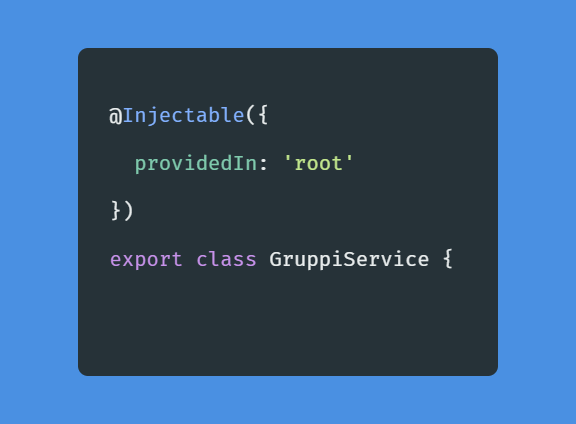
\includegraphics[scale=0.2]{progettazione/injectable.png}
          %     \caption{Esempio di creazione di un servizio}
          % \end{figure}
          \begin{lstlisting}[style = Java, caption = {Esempio di creazione di un servizio}]
@Injectable({
    providedIn: `root',
    })
    export class GruppiService {
\end{lstlisting}
    \item  si inietta il servizio e lo si utilizza ovunque sia necessario.
          \cite{site-dependency-injection-angular}
          % \begin{figure}[H] 
          %     \centering 
          %     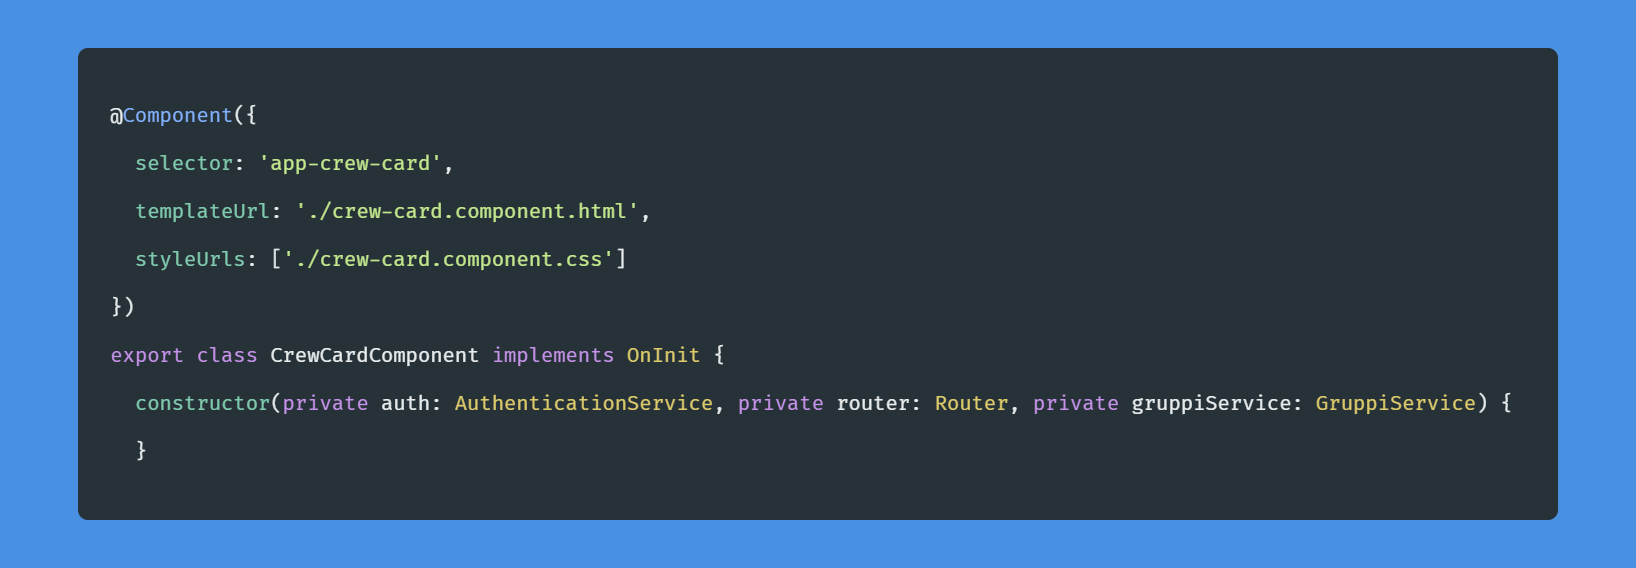
\includegraphics[scale=0.2]{progettazione/injected-service.png}
          %     \caption{Esempio di \textit{constructor injection}}
          % \end{figure}
          \begin{lstlisting}[style= Java, caption = {Esempio di \textit{constructor injection}}]
@Component({
    selector: `app-crew-card',
    templateUrl: `./crew-card.component.html',
    styleUrls: [`./crew-card.component.css'],
    })
export class CrewCardComponent implements OnInit {

    constructor(private auth: AuthenticationService, private router: Router,private gruppiService: GruppiService){

    }
}
\end{lstlisting}
\end{itemize}
\subsection{Singleton}
\label{sub:Singleton}
Angular e Spring integrano fra i loro \textit{pattern} il \class{Singleton},
che viene implementato mediante l'utilizzo della
\nameref{sub:Dependency-Injection}.\\
Utilizzando questo \textit{pattern} è stato possibile creare una sola istanza
di una classe, potendola utilizzare fra i vari servizi e componenti.\\
L'utilizzo del \textit{pattern Singleton}, tuttavia, potrebbe violare il
\gls{SRP}, rendendolo un \textit{anti-pattern}. Nel contesto del progetto di
\textit{stage}, questo \textit{pattern} è stato utilizzato per le classi di
tipo \textit{Controller}, \textit{Service} e \textit{Repository}. In questo
caso il suo utilizzo è necessario in quanto sarebbe logicamente sbagliato avere
più istanze per il tipo di classi sopra citate. \cite{site-singleton}

\subsection{Feature Service}
Questo \textit{pattern} è utilizzato da Angular per estrarre da una classe di
tipo \textit{Component} la sua relativa logica, che può essere per esempio la
visualizzazione dei dettagli di un gruppo.\\
Mediante l'utilizzo del \textit{pattern} \nameref{sub:Singleton} e
\nameref{sub:Dependency-Injection} è possibile utilizzare i vari componenti in
tutti i componenti dell'applicazione. \cite{site-feature-modules}
\subsection{Lazy Loading}
Questo \textit{pattern} è utilizzato da Angular per caricare i moduli solo nel
momento in cui effettivamente vengono utilizzati, ottenendo così bassa la
quantità di dati scaricata dall'utente iniziale e una diminuzione del tempo
necessario al caricamento dell'applicazione.\\
Viene utilizzato questo \textit{pattern} per la gestione del \textit{routing},
associando ad una specifica \textit{view} dell'applicazione un \textit{path} di
navigazione presente nella \gls{URL}.\cite{site-lazy-loading}
% \begin{figure}[H] 
%     \centering 
%     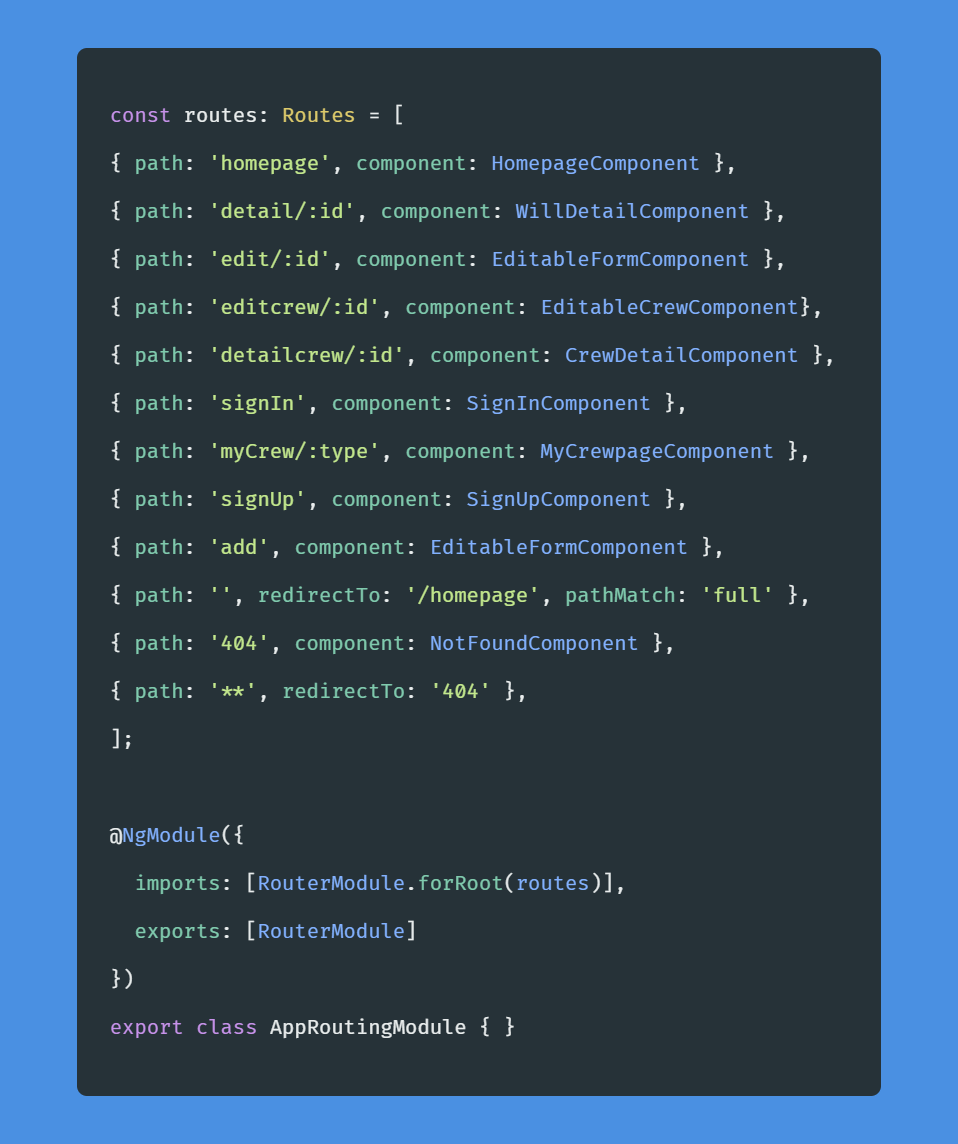
\includegraphics[scale=0.3]{progettazione/routing.png}
%     \caption{Implementazione del \textit{pattern} \textit{Lazy loading} nel \textit{AppRoutingModule}}
% \end{figure}\

\begin{lstlisting}[style=Java, caption = {Implementazione del \textit{pattern} \textit{Lazy loading} nel \texttt{AppRoutingModule}}]
const routes: Routes = [
    { path: `homepage', component: HomepageComponent },
    { path: `detail/:id', component: WillDetailComponent },
    { path: `edit/:id', component: EditableFormComponent },
    { path: `editcrew/:id', component: EditableCrewComponent},
    { path: `detailcrew/:id', component: CrewDetailComponent },
    { path: `signIn', component: SignInComponent },
    { path: `myCrew/:type', component: MyCrewpageComponent },
    { path: `signUp', component: SignUpComponent },
    { path: `add', component: EditableFormComponent },
    { path: `', redirectTo: `/homepage', pathMatch: `full' },
    { path: `404', component: NotFoundComponent },
    { path: `**', redirectTo: `404' }
    ];
    
    @NgModule({
        imports: [RouterModule.forRoot(routes)],
        exports: [RouterModule]
    })
    export class AppRoutingModule { }  
\end{lstlisting}

\subsection{Observer}
Gli \class{Observable} forniscono supporto per il passaggio di messaggi tra le
parti dell'applicazione. Sono usati frequentemente in Angular e sono una
tecnica per la gestione ad eventi e la programmazione asincrona.\\
Il \textit{pattern} \class{Observer} è un \textit{design pattern} in cui un
oggetto, chiamato \texttt{Subject}, contiene una lista di suoi osservatori,
chiamati \texttt{Observers}, e li notifica automaticamente ai cambiamenti di
stato.\\
Gli \textit{Observable} sono dichiarativi, ovvero viene definita una funzione
che non viene eseguita fino a quando un \textit{Observer} si sottoscrive ad
esso. L'\textit{Observer} viene quindi notificato al completamento della
funzione, e il tipo di ritorno di un \textit{Observable} può cambiare in base
al contesto, che nel caso nel progetto di \textit{stage} è stato
prevalentemente di tipo HTTP \textit{response}. \cite{site-observable}\\
% \begin{figure}[H] 
%     \centering 
%     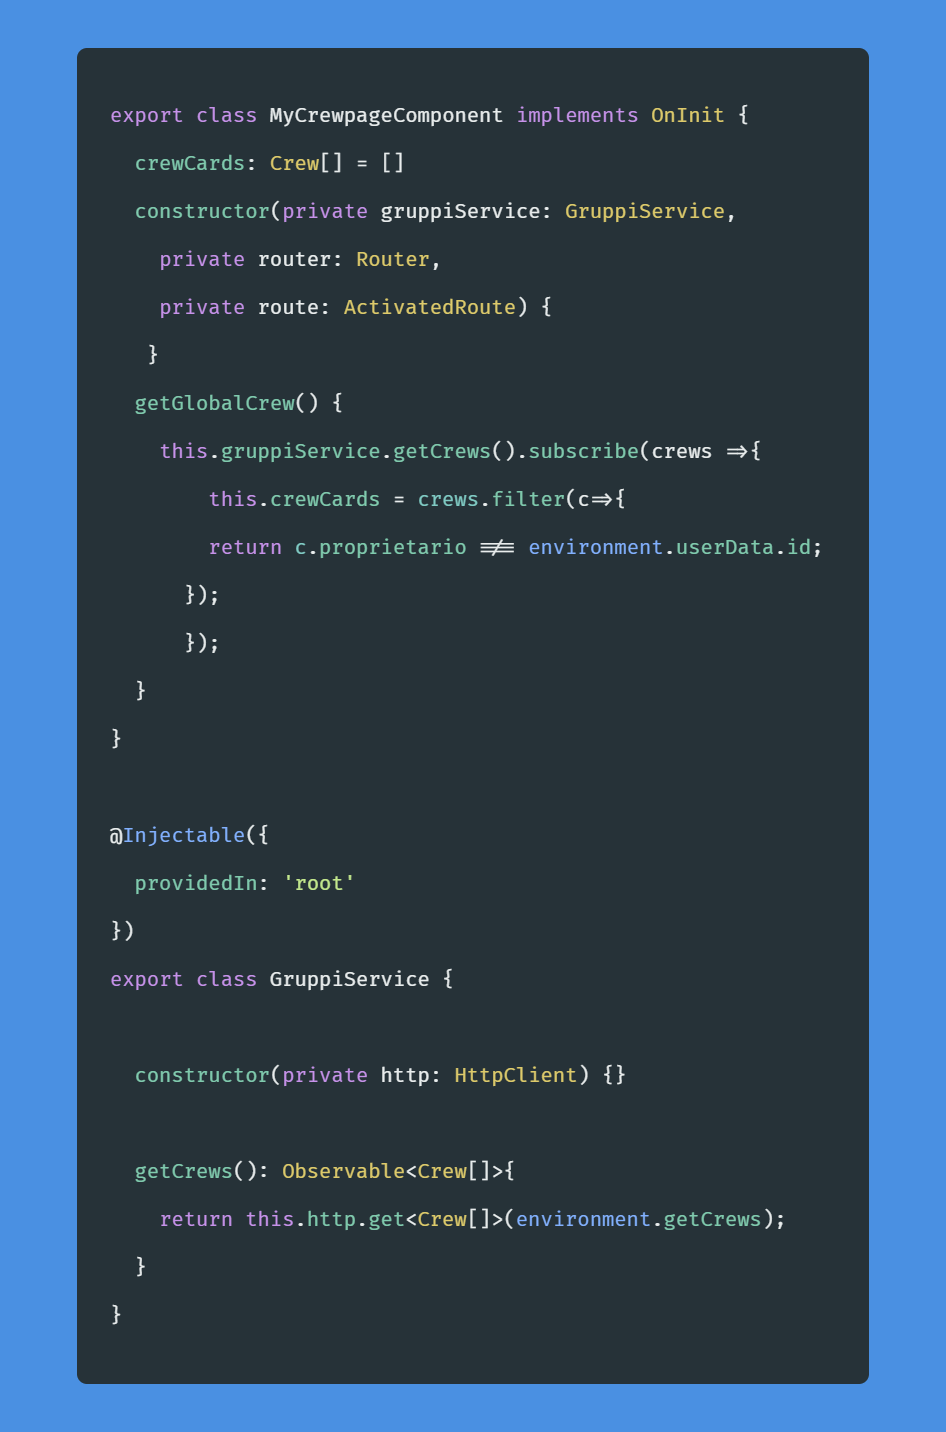
\includegraphics[scale=0.28]{progettazione/subscribe-example.png}
%     \caption{Esempio implementazione \textit{pattern Observer}}
% \end{figure}
\begin{lstlisting}[style=Java, caption = {Esempio implementazione \textit{pattern Observer}}]
export class MyCrewpageComponent implements OnInit {
    crewCards: Crew[] = [];
    constructor(
        private gruppiService: GruppiService,
        private router: Router,
        private route: ActivatedRoute) {
    }
    getGlobalCrew() {
        this.gruppiService.getCrewsOfUser().subscribe((crews) => {
          this.gruppiService.getCrews().subscribe((crews2) => {
            this.crewCards = crews2.filter((c) => {
              let toReturn: boolean = true;
              for (let crew of crews){
                if (crew.id == c.id){
                  toReturn = false;
                  break;
                }
              }
              return toReturn;
            });
          });
        });
    }
}

@Injectable({
  providedIn: `root',
})
export class GruppiService {
  constructor(private http: HttpClient) {}

  getCrews(): Observable<Crew[]> {
    return this.http.get<Crew[]>(environment.getCrews);
  }
}
\end{lstlisting}

%**************************************************************
\section{Codifica}
\subsection{Back end}
\subsubsection{Gruppi service}
\myparagraph{Crew}
\label{par:Crew}
Questa classe rappresenta i gruppi. La tabella che mappa la classe nel
\textit{database} è rappresentata nella figura \ref{img:Crew-tabella}. Per
aggiungere o modificare un gruppo è necessario rappresentare la classe in
formato JSON, come in figura \ref{img:Crew-classe-json}. Per creare un nuovo
gruppo è necessario specificare almeno i campi \texttt{nome, proprietario,
    latitudine} e \texttt{longitudine}.

\begin{figure}[H]
    \centerline{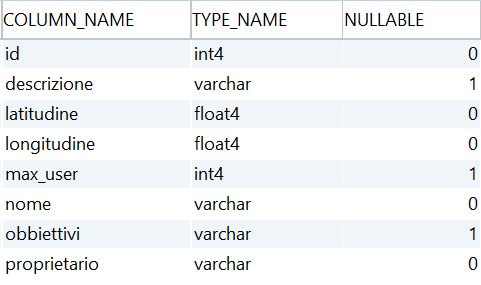
\includegraphics[scale=0.7]{codice/crew-table.png}}
    \caption{Tabella \texttt{Crew}}
    \label{img:Crew-tabella}
\end{figure}

% \begin{figure}[H]
%     \centerline{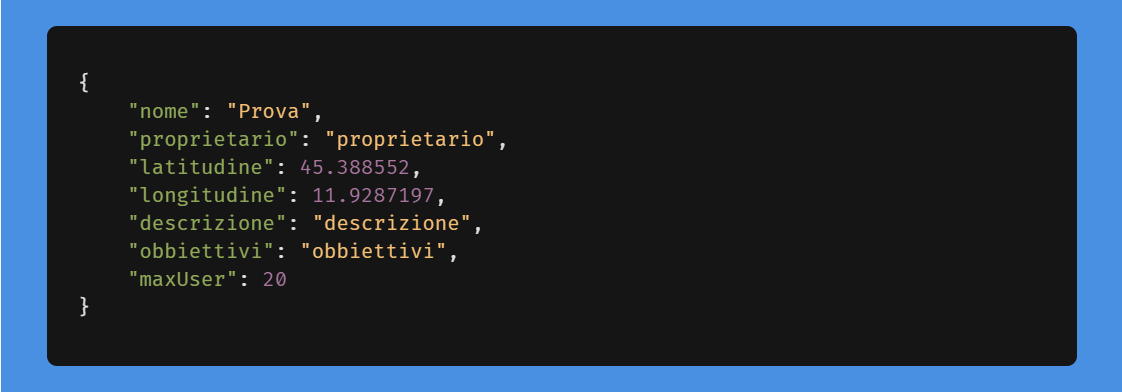
\includegraphics[scale=0.3]{codice/crew-classe-json.png}}
%     \caption{Rappresentazione JSON della classe \texttt{Crew}}
%     \label{img:Crew-classe-json}
% \end{figure}
\begin{lstlisting}[language=json,firstnumber=1, caption={Rappresentazione JSON della classe \texttt{Crew}}, label={img:Crew-classe-json}]
{
    "nome": "Prova",
    "proprietario": "proprietario",
    "latitudine": 45.388552,
    "longitudine": 11.9287197,
    "descrizione": "descrizione",
    "obbiettivi": "obbiettivi",
    "maxUser": 20
}  
\end{lstlisting}

\myparagraph{GruppiController}
\label{par:GruppiController}
% TODO: aggiungere immagine della classe
Classe che permette di esporre le \gls{API} mappate nel \textit{path}
\texttt{/gruppi}.
L'annotazione \code{@RestController} permette di creare un \textit{controller
    Restful}, e l'oggetto da restituire viene serializzato automaticamente in
JSON
e restituito all'oggetto di risposta HTTP.
\subparagraph*{Metodi principali}
\begin{itemize}
    \item \class{getAllGruppi}: gestisce la chiamata che visualizza tutti i
          gruppi.\\ \mappaturaemetodo{/}{GET};
    \item \class{getGruppo}:  gestisce la chiamata che visualizza un gruppo
          specifico. \\ \mappaturaemetodo{/\{id\}}{GET};
    \item \class{getUtentiByGruppo}: gestisce la chiamata che visualizza gli
          utenti appartenenti ad un gruppo. \\
          \mappaturaemetodo{/\{idCrew\}/utenti}{GET};
    \item \class{createGruppo}: gestisce la chiamata che inserisce una nuovo
          gruppo. È necessario specificare i dati del gruppo da inserire nel
          \textit{body} della chiamata HTTP, come in figura
          \ref{img:Crew-classe-json}.
          \\ \mappaturaemetodo{/inserisci}{POST};
    \item \class{modifyGruppo}: gestisce la chiamata che modifica un gruppo. È
          necessario specificare i dati del gruppo da modificare nel
          \textit{body} della
          chiamata HTTP, come in figura \ref{img:Crew-classe-json}. I campi non
          specificati non verranno modificati. \\
          \mappaturaemetodo{/modifica/\{idCrew\}}{PUT};
    \item \class{getUsciteByGruppo}: gestisce la chiamata che visualizza le
          uscite di una gruppo.\\ \mappaturaemetodo{/\{idCrew\}/uscite}{GET};
    \item \class{deleteGruppo}: gestisce la chiamata che elimina un gruppo. \\
          \mappaturaemetodo{/elimina/\{idCrew\}}{DELETE};
    \item \class{getGruppiUtente}: gestisce la chiamata che richiede tutti i
          gruppi a cui appartiene un utente. \\
          \mappaturaemetodo{/utente/\{idUtente\}}{GET};
    \item \class{addUtenteToGruppo}: gestisce la chiamata che permette ad un
          utente di unirsi ad un gruppo. \\
          \mappaturaemetodo{/\{idCrew\}/aggiungi/utente/\{idUtente\}}{POST};
    \item \class{removeUtenteFromGruppo}: gestisce la chiamata che permette ad
          un utente di rimuoversi da un gruppo. \\
          \mappaturaemetodo{/\{idCrew\}/elimina/utente/\{idUtente\}}{DELETE};
    \item \class{addUscitaToGruppo}:  gestisce l'aggiunta di un'uscita ad un
          gruppo. \\
          \mappaturaemetodo{/\{idCrew\}/aggiungi/uscita/\{idUscita\}}{POST};
    \item \class{removeUscitaFromGruppo}: gestisce l'eliminazione di un'uscita
          ad un gruppo. \\
          \mappaturaemetodo{/\{idCrew\}/elimina/uscita/\{idUscita\}}{DELETE}.
\end{itemize}

\myparagraph{GruppiService}
% TODO: aggiungere immagine della classe
Classe responsabile della \textit{business logic} del \gls{microservizio}.  \\
Siccome fornisce funzionalità di \textit{business}, questa classe è annotata
con l'annotazione \code{@Service}, e funge da intermediario fra la classe
\nameref{par:GruppiController} e  il \gls{DAO}, ovvero le classi
\hyperref[CrewRepository]{CrewRepository},
\hyperref[JointUtentiCrewRepository]{JointUtentiCrewRepository} e
\hyperref[JointUsciteCrewRepository]{JointUsciteCrewRepository}. \\
I metodi di questa classe hanno gli stessi nomi e funzione dei metodi presenti
in \nameref{par:GruppiController}.

\myparagraph{Repository}
\label{Repository}
Interfacce con funzionalità \gls{JPA} che permettono di mappare una classe in
una tabella di un \textit{database} relazionale, svolgendo anche il compito
\gls{EntityManager}, effettuando l'accesso agli oggetti ed eseguendo operazioni
\gls{CRUD} sui dati immagazzinati nelle tabelle del \textit{database}.\\
Tutte queste interfacce estendono l'interfaccia \code{JpaRepository<T,ID>},
dove \texttt{T} è il tipo della classe da mappare, ed \texttt{ID} è il tipo
dell'identificativo della classe mappata.\\
L'interfaccia \texttt{JpaRepository} permette di creare le \textit{query} a
partire dal nome del metodo, senza doverlo necessariamente implementare.\\
Il meccanismo che permette di generare le \textit{query} integrato
nell'infrastruttura JPA Spring Data è utile per creare \textit{query} vincolate
sulle entità del \textit{repository}. Questo meccanismo rimuove i prefissi
\texttt{find...By}, \texttt{read...By} e \texttt{get...By} dal metodo ed
effettua il \textit{parsing} della funzione alla ricerca dei nomi delle
proprietà dell'entità mappata nel \texttt{JpaRepository}, come nel seguente
esempio:
\begin{center}
    \code{List<JointUsciteCrew> findAllByIdCrew(int idCrew);}
\end{center}
in cui \texttt{idCrew} è una proprietà dell'entità \texttt{JointUsciteCrew}.\\
Le proprietà inserite nel nome del metodo possono essere concatenate con
\textit{And} e \textit{Or}, ma anche con operatori come \textit{Between},
\textit{LessThan}, \textit{GreaterThan}, \textit{Like}. \\
Un esempio è il seguente:
\begin{center}
    \code{Long deleteByIdUscitaAndIdCrew (int idUscita, int idCrew);}
\end{center}
È possibile applicare l'ordinamento statico aggiungendo una clausola
\textit{OrderBy} al metodo di \textit{query} facendo riferimento ad una
proprietà, come nel seguente caso:
\begin{center}
    \code{List<Crew> findByOrderById()};
\end{center}
Ci sono tre \textit{repository} nel \gls{microservizio}:
\nameref{JointUsciteCrewRepository}, \nameref{JointUtentiCrewRepository} e
\nameref{CrewRepository}.
\mysubparagraph{JointUsciteCrewRepository}
\label{JointUsciteCrewRepository}
Classe di \textit{repository} che contiene le uscite di un gruppo. Ogni
qualvolta un utente aggiunge un'uscita, essa viene aggiunta alle uscite di
tutti i gruppi a cui appartiene. Viceversa quando viene eliminata un'uscita
viene eliminata dalle uscite di tutti i gruppi.\\
Un accorgimento che è stato fatto è che quando viene rimosso un gruppo, tutte
le uscite associate a quel gruppo vengono rimosse da questa tabella (n.b. le
uscite non vengono eliminate dalla tabella \texttt{Uscite} presente nel
\textit{database}, vengono solo eliminate le voci relative nella tabella
\texttt{joint\_uscite\_crew}).
\subsubparagraph{Metodi}
\begin{itemize}
    \item \class{List<JointUsciteCrew> findAllByIdCrew(int idCrew)}:
          restituisce tutte le occorrenze in base all'id del gruppo;
    \item \class{Long deleteByIdUscitaAndIdCrew (int idUscita, int idCrew)}:
          elimina le occorrenze in base all'id del gruppo e all'id dell'uscita.
          Ritorna
          il numero di occorrenze eliminate (che sono al più una);
    \item \class{JointUsciteCrew getByIdUscitaAndIdCrew(int idUscita, int
              idCrew)}: restituisce un'occorrenza in base all'id dell'uscita e
          all'id del
          gruppo;
    \item \class{Long deleteByIdCrew(int idCrew)}: elimina tutte le occorrenze
          in base all'id del gruppo. Ritorna il numero di occorrenze eliminate;
    \item \class{void deleteByIdUscita(int idUscita)}: elimina tutte le
          occorrenze in base all'id dell'uscita.
\end{itemize}

\mysubparagraph{JointUtentiCrewRepository}
% TODO: aggiungere immagine della classe
\label{JointUtentiCrewRepository}
Classe di \textit{repository} che contiene le partecipazioni degli utenti ai
gruppi. \\
Come in \hyperref[JointUsciteCrewRepository]{JointUsciteCrewRepository}, quando
viene eliminato un utente vengono rimosse le partecipazioni degli utenti a
tutti i gruppi a cui partecipava. Tuttavia è stato deciso di non eliminare i
gruppi creati da un utente nel caso di eliminazione, in quanto i gruppi non
sono strettamente associati al suo creatore, ma sono delle entità indipendenti.
\subsubparagraph{Metodi}
\begin{itemize}
    \item \class{List<JointUtentiCrew> findAllByIdUtente(String utenteId)}:
          restituisce tutte le occorrenze in base all'id dell'utente;
    \item \class{void deleteByIdUtenteAndIdCrew(String idUtente, int idCrew)}:
          elimina le occorrenze in base all'id dell'utente e all'id del gruppo;
    \item \class{JointUtentiCrew getByIdUtenteAndIdCrew(String idUtente, int
              idCrew)}: restituisce un'occorrenza in base all'id dell'utente e
          all'id del
          gruppo;
    \item \class{Long deleteByIdCrew(int idCrew)}: elimina tutte le occorrenze
          in base all'id del gruppo. Ritorna il numero di occorrenze eliminate;
    \item \class{List<JointUtentiCrew> findAllByIdCrew(int id)}: restituisce
          tutte le occorrenze in base all'id del gruppo;
    \item \class{void deleteByIdUtente(String idUtente)}: elimina tutte le
          occorrenze in base all'id dell'utente.

\end{itemize}

\mysubparagraph{CrewRepository}
% TODO: aggiungere immagine della classe
\label{CrewRepository}
Classe di \textit{repository} che contiene i dettagli dei gruppi. \\
\subsubparagraph{Metodi}
\begin{itemize}
    \item \class{List<Crew> findByOrderById()}: restituisce tutti i gruppi
          ordinati per id;
    \item \class{Crew findById(int id)}: restituisce un gruppo in base al suo
          id;
    \item \class{Long deleteById(int id)}: elimina un'occorrenza in base
          all'id. Ritorna uno se avviene un'eliminazione, zero altrimenti.
\end{itemize}

\subsubsection{Uscite Service}
In questo \gls{microservizio} sono state effettuate le seguenti modifiche:
\begin{itemize}
    \item è stato aggiunto un campo booleano \texttt{visGlobale} alla classe
          \texttt{Uscita} che permette di specificare se l'uscita sarà visibile
          da tutti
          gli utenti oppure soltanto dagli utenti appartenenti agli stessi
          gruppi;
    \item è stato aggiunto al metodo \texttt{createUscita} presente nella
          classe \texttt{UsciteController} la possibilità di inserire nel corpo
          per la
          creazione dell'uscita il campo che specifica il tipo di visibilità
          desiderata.
          \\
          Nello stesso metodo è stata anche inserita una chiamata HTTP che
          aggiunge
          l'uscita appena creata al \textit{repository}
          \hyperref[JointUsciteCrewRepository]{JointUsciteCrewRepository};
    \item è stato aggiunto al metodo \texttt{eliminaUscita} una chiamata HTTP
          che rimuove l'uscita dal \textit{repository}
          \hyperref[JointUsciteCrewRepository]{JointUsciteCrewRepository};
    \item è stato aggiunto un metodo \texttt{modificaVisibilita}  alla classe
          \texttt{UsciteController} che permette di modificare la visibilità
          dell'uscita.
          Questo metodo viene mappato in
          \texttt{uscite/modifica/visibilità/\{id\}},
          ed \texttt{id} specifica l'\texttt{id} del gruppo del quale si vuole
          modificare
          la visibilità. Il verbo HTTP della chiamata è di tipo PUT;
    \item è stato aggiunto un metodo \texttt{getAllUsciteGlobali}  alla classe
          \texttt{UsciteController} che permette di ricevere tutte le uscite
          che hanno il
          campo \code{visGlobale = true}. \\
          Questo metodo viene mappato in \texttt{uscite/globali}, ed il verbo
          HTTP
          della chiamata è di tipo GET.
\end{itemize}

\subsubsection{Api Gateway}
È stato implementato un \textit{Spring Cloud Gateway} applicando dei filtri
alle chiamate per verificare se è presente e valido il \textit{token} per
l'autenticazione  presente nell'\textit{header} della richiesta HTTP.
Per fare ciò è stato creata una classe \texttt{AuthFilter} che estende
l'interfaccia \texttt{AbstractGatewayFilterFactory} ed implementa il metodo
astratto \code{GatewayFilter apply(C config)} presente nella
\textit{superclasse}. In questa funzione viene letta la richiesta in entrata
viene verificata l'autenticazione.

% \begin{figure}[H] 
%     \centerline{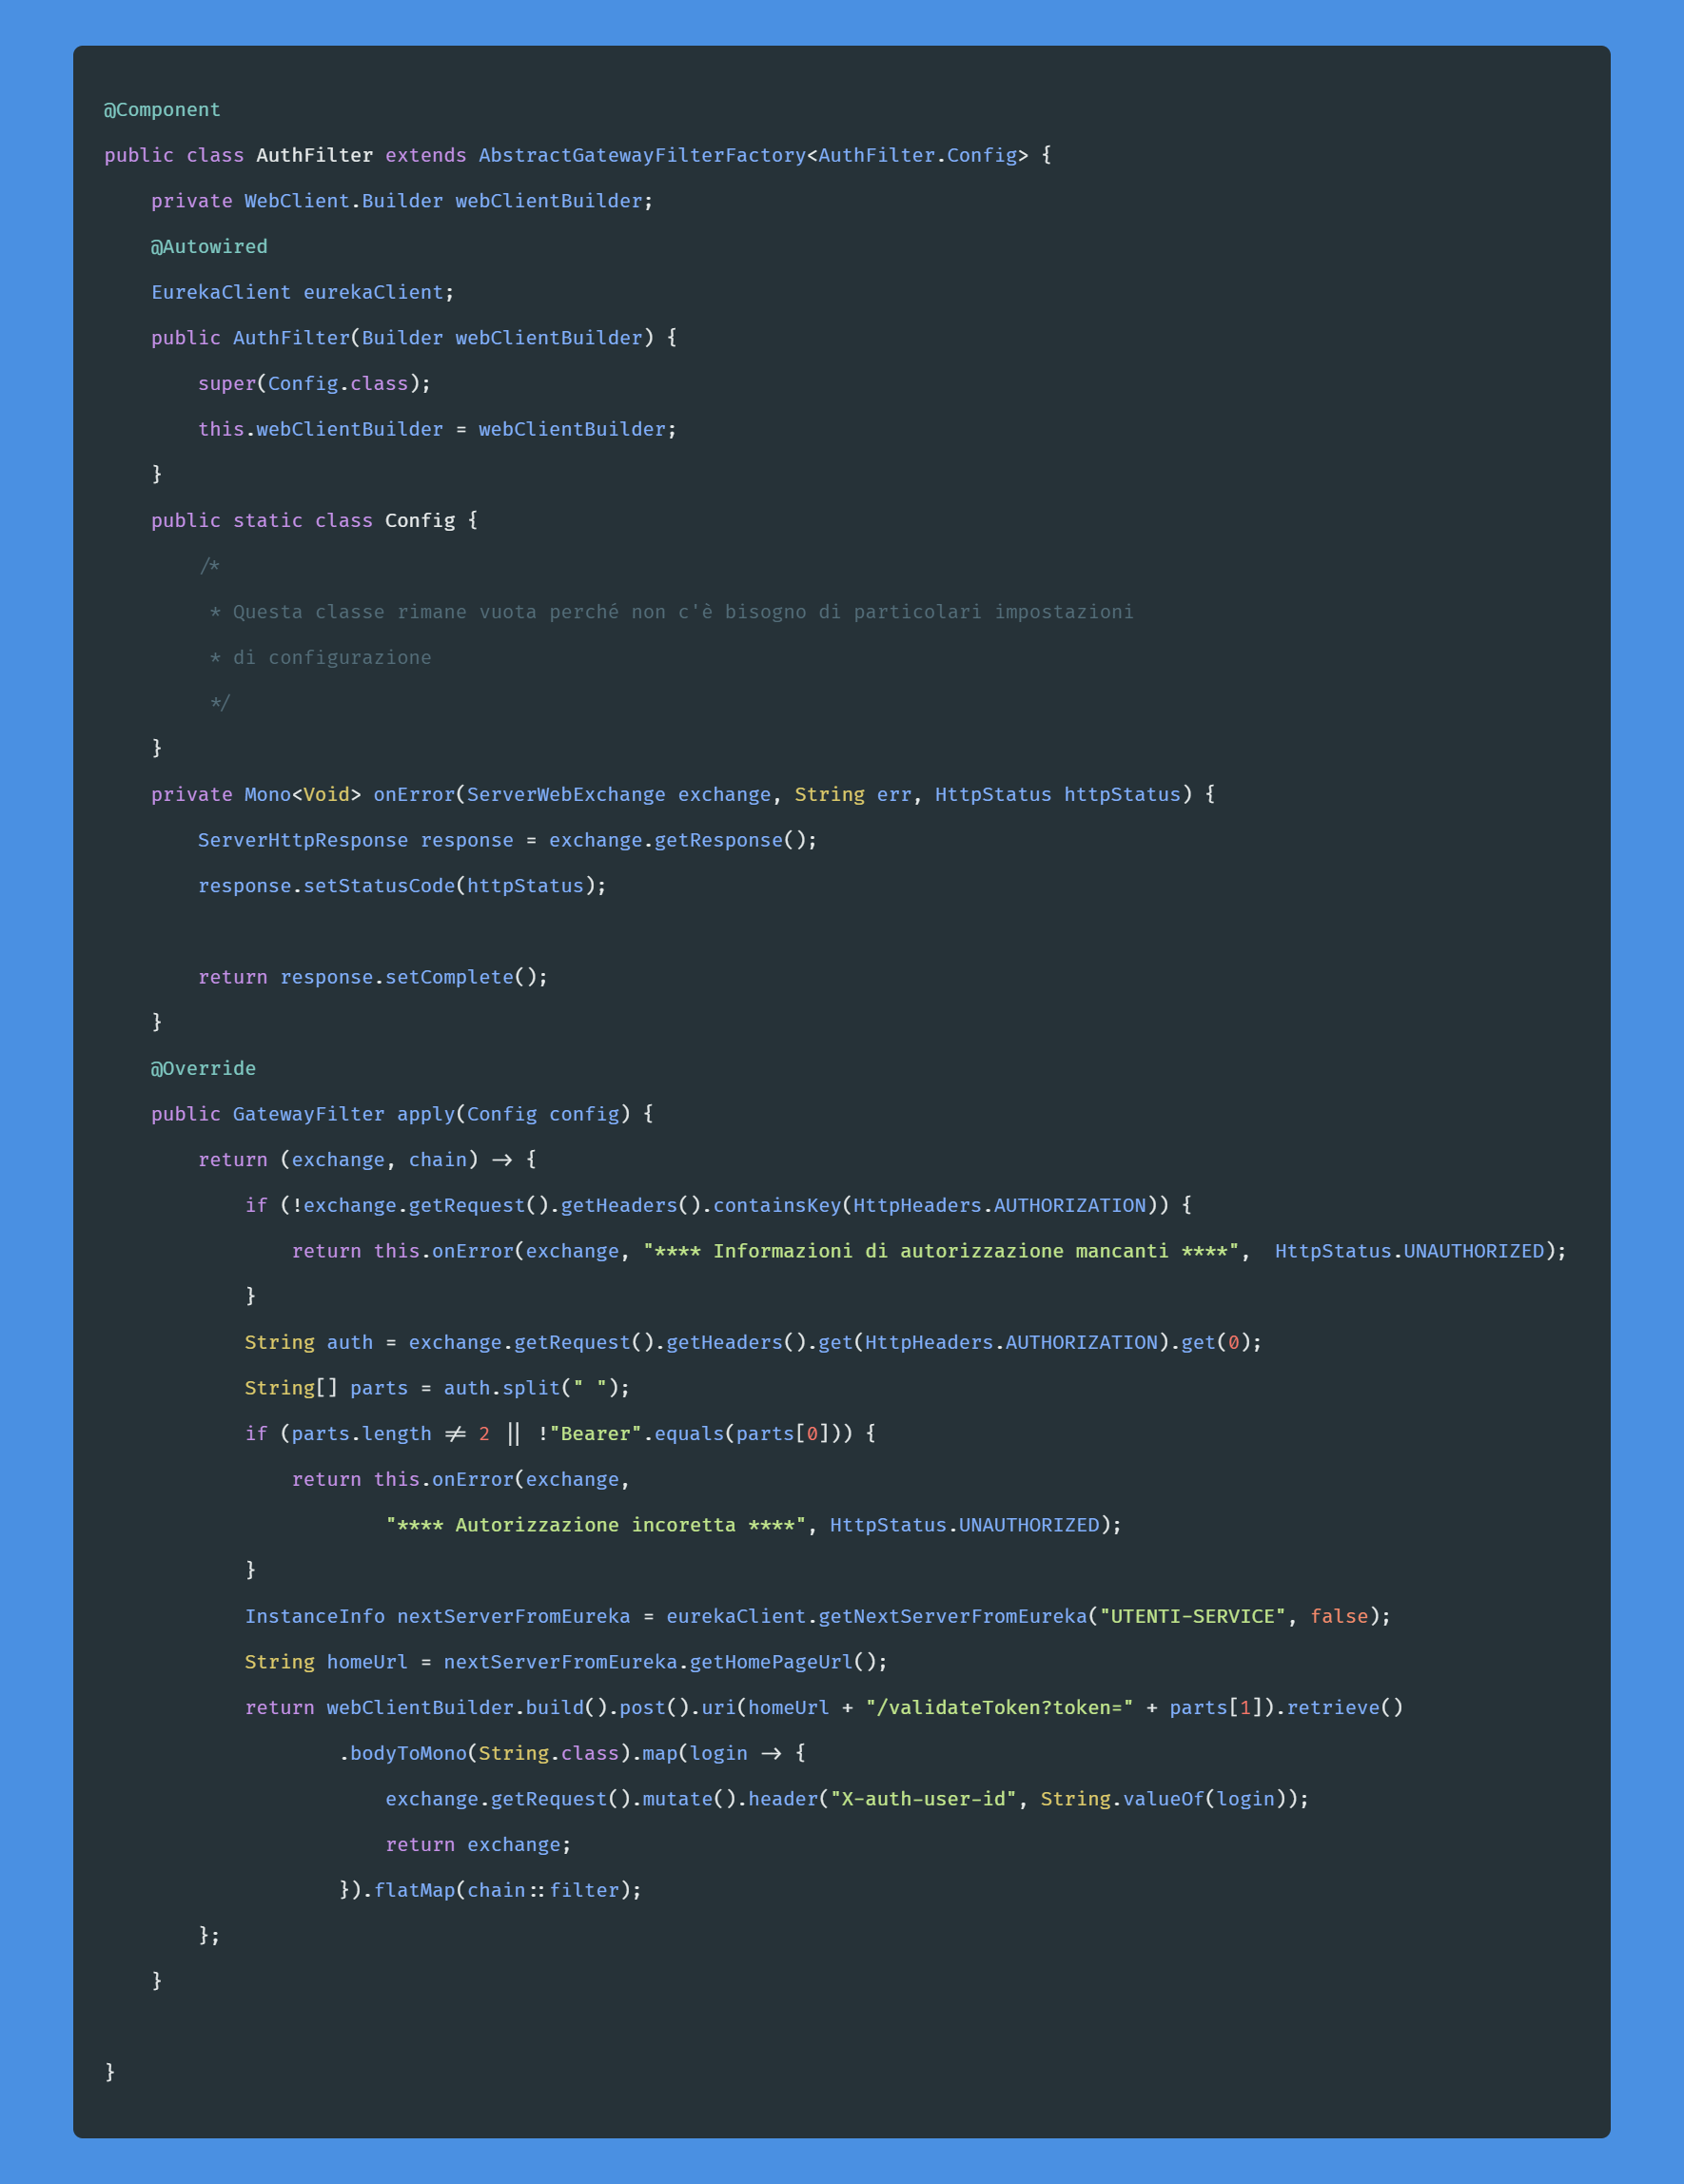
\includegraphics[scale=0.25]{codice/AuthFilter.png}}
%     \caption{Implementazione della classe \textit{AuthFilter}}
% \end{figure}
\begin{lstlisting}[style = Java, caption = {Implementazione della classe \textit{AuthFilter}}]
    @Component
    public class AuthFilter extends AbstractGatewayFilterFactory<AuthFilter.Config> {
    
        private WebClient.Builder webClientBuilder;
    
        @Autowired
        EurekaClient eurekaClient;
    
        public AuthFilter(Builder webClientBuilder) {
            super(Config.class);
            this.webClientBuilder = webClientBuilder;
        }
    
        public static class Config {
            /*
             * Questa classe rimane vuota perche non c'e bisogno di particolari * impostazioni
             * di configurazione
             */
        }
    
        private Mono<Void> onError(ServerWebExchange exchange, String err, HttpStatus httpStatus) {
            ServerHttpResponse response = exchange.getResponse();
            response.setStatusCode(httpStatus);
    
            return response.setComplete();
        }
        @Override
        public GatewayFilter apply(Config config) {
            return (exchange, chain) -> {
                if (!exchange.getRequest().getHeaders().containsKey(HttpHeaders.AUTHORIZATION)) {
                    return this.onError(exchange, "**** Informazioni di autorizzazione mancanti ****",  HttpStatus.UNAUTHORIZED);
                }
                String auth = exchange.getRequest().getHeaders().get(HttpHeaders.AUTHORIZATION).get(0);
                String[] parts = auth.split(" ");
                if (parts.length != 2 || !"Bearer".equals(parts[0])) {
                    return this.onError(exchange, 
                            "**** Autorizzazione incoretta ****", HttpStatus.UNAUTHORIZED);
                }
                InstanceInfo nextServerFromEureka = eurekaClient.getNextServerFromEureka("UTENTI-SERVICE", false);
                String homeUrl = nextServerFromEureka.getHomePageUrl();
                return webClientBuilder.build().post().uri(homeUrl + "/validateToken?token=" + parts[1]).retrieve()
                        .bodyToMono(String.class).map(login -> {
                            exchange.getRequest().mutate().header("X-auth-user-id", String.valueOf(login));
                            return exchange;
                        }).flatMap(chain::filter);
            };
        }
    
    }
\end{lstlisting}

\noindent Infine, è stata utilizzata la seguente configurazione dello
\textit{Spring Cloud Gateway} nel file \texttt{configuration.yml}.

\begin{lstlisting}[language = yaml, caption = {Configurazione dello \textit{Spring Cloud Gateway} nel file \texttt{application.yml} del microservizio \texttt{API Gateway}}]
    spring:
    application:
      name: API-GATEWAY-SERVICE
    main:
      allow-bean-definition-overriding: true
    cloud:
      gateway:
        discovery.locator.enabled: true
        routes:
          - id: utenti
            uri: lb://UTENTI-SERVICE
            predicates:
              - Path= /utenti/^**,^ /signin, /signup, /validateToken
            filters:
              - AuthFilter
          - id: posizioni
            uri: lb://POSIZIONI-SERVICE
            predicates:
              Path=/posizioni/^**^
            filters:
              - AuthFilter
          - id: uscite
            uri: lb://USCITE-SERVICE
            predicates:
              Path=/uscite/^**^
            filters:
              - AuthFilter
          - id: gruppi
            uri: lb://GRUPPI-SERVICE
            predicates:
              Path=/gruppi/^**^
            filters:
              - AuthFilter
        default-filters:
          - DedupeResponseHeader=Access-Control-Allow-Credentials Access-Control-Allow-Origin
        globalcors:
          corsConfigurations:
          `[/**]':
                allowedOrigins: "http://localhost:4200/"
                allowedMethods: "*"
                allowedHeaders: "*"  
\end{lstlisting}

% \begin{figure}[H] 
%     \centering
%     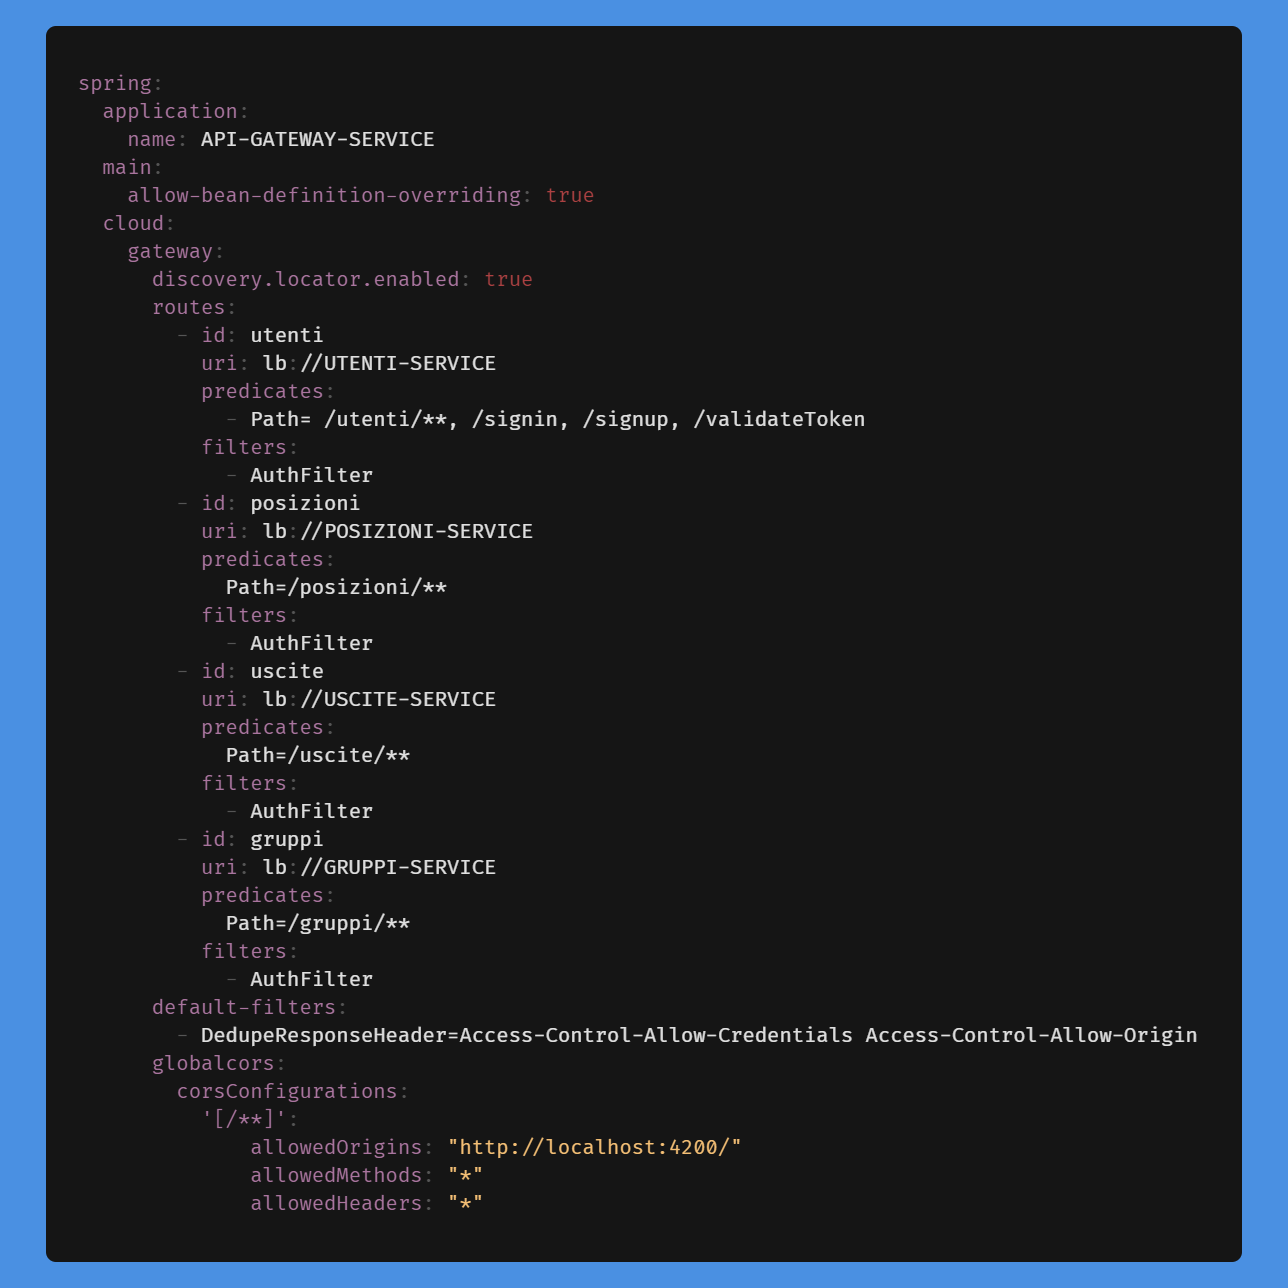
\includegraphics[width=1\columnwidth]{codice/application.yml-API-Gateway.png} 
%     \caption{Configurazione dello \textit{Spring Cloud Gateway} nel file \texttt{application.yml} del microservizio \textit{API Gateway}}
% \end{figure}

\subsection{Eureka Server}
Questo \gls{microservizio} contiene solo una classe al suo interno, che è la
classe che viene generata automaticamente quando si inizializza un progetto con
Spring. L'unica cosa aggiunta alla classe è l'annotazione
\code{@EnableEurekaServer}, che permette di  attivare la l'\gls{Eureka Server}
come specificato nel file \texttt{application.yml}.

% \begin{figure}[H] 
%     \centering
%     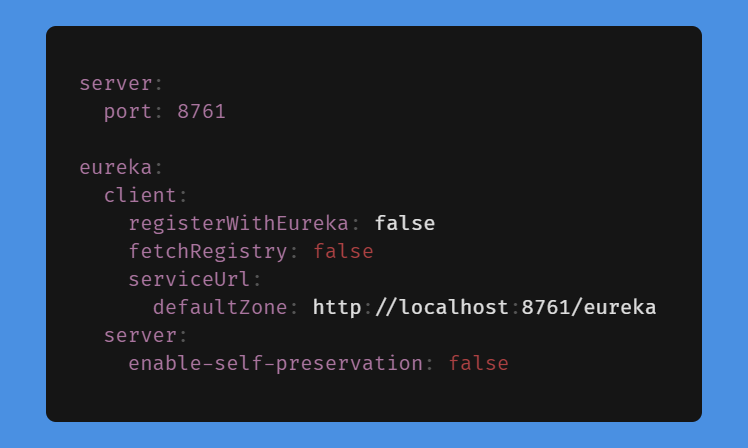
\includegraphics[width=1\columnwidth]{codice/application.yml-Eureka.png} 
%     \caption{File \texttt{application.yml} del microservizio \textit{Eureka} Server}
% \end{figure}
\begin{lstlisting}[language = yaml, caption = {File \texttt{application.yml} del microservizio \texttt{Eureka Server}}]
server:
    port: 8761
eureka:
    client:
        registerWithEureka: false 
        fetchRegistry: false
        serviceUrl:
        defaultZone: http://localhost:8761/eureka
    server:
        enable-self-preservation: false
\end{lstlisting}
\noindent Nella \textit{Main class} di tutti i \glspl{microservizio}  è stata
aggiunta l'annotazione \code{@EnableEurekaClient}, che permette di registrarsi
all'\gls{Eureka Server} in base a quanto specificato nel file
\texttt{application.properties}.\\

\begin{lstlisting}[style=Docker, caption = {Configurazione per la registrazione di un microservizio all'\texttt{Eureka Server} nel file \texttt{application.properties}}]
eureka.client.service-url.defaultZone: http:^//^localhost:8761/eureka
eureka.client.register-with-eureka=true
eureka.client.fetch-registry=true
\end{lstlisting}

\subsubsection{Docker}
Per ogni \gls{microservizio} è stato creato un file \texttt{Dockerfile}
contenente le operazioni da effettuare per la creazione di un'immagine Docker.
Tutti i \texttt{Dockerfile} hanno la seguente struttura:

\begin{lstlisting}[style=Docker]
FROM openjdk:11
ARG JAR_FILE=target *.jar
COPY ${JAR_FILE} nome_microservizio.jar
ENTRYPOINT ["java","-jar","nome_microservizio.jar"]
\end{lstlisting}

Per eseguire ogni \gls{container} nello stesso \textit{network} è stato creato
un file \texttt{docker-compose.yml} in cui vengono specificate le immagini
Docker da avviare.
\subsection{Front end}
In questa sezione verranno descritte solo le maschere, componenti e servizi
modificati in maniera rilevante o creati. Tutto ciò che era già presente nella
\textit{web app} non verrà descritta.
\subsubsection{Maschere}
\myparagraph{Homepage}
Questa pagina permette ad un utente autenticato di visualizzare le \gls{will}
visibili da tutti gli utenti, le \gls{will} create dall'utente e le \gls{will}
dei gruppi a cui partecipa.
\begin{figure}[H]
    \centering
    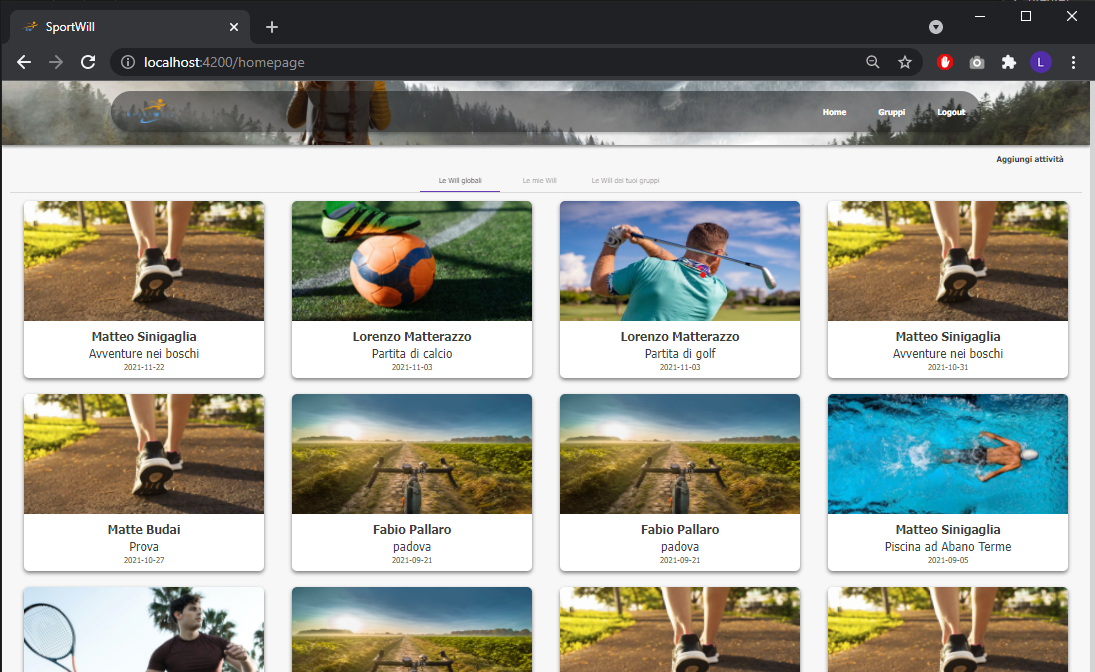
\includegraphics[scale=0.6]{sito/homepage-will-globali.png}
    \caption{Pagina di homepage}
\end{figure}
\mysubparagraph{Componenti utilizzati}
\begin{itemize}
    \item \hyperref[par:HomepageComponent]{HomepageComponent}
          % \item \hyperref[par:CrewCard]{CrewCard}
\end{itemize}
% \mysubparagraph{Servizi}
% \begin{itemize}
%     \item \hyperref[par:GruppiService]{GruppiService}
%     \item \hyperref[par:WillDataService]{WillDataService}
% \end{itemize}

\myparagraph{Gruppi dell'utente}
\label{par:Gruppi dell'utente}
Questa pagina permette ad un utente autenticato di visualizzare i gruppi creati
o a cui partecipa un utente.
\begin{figure}[H]
    \centering
    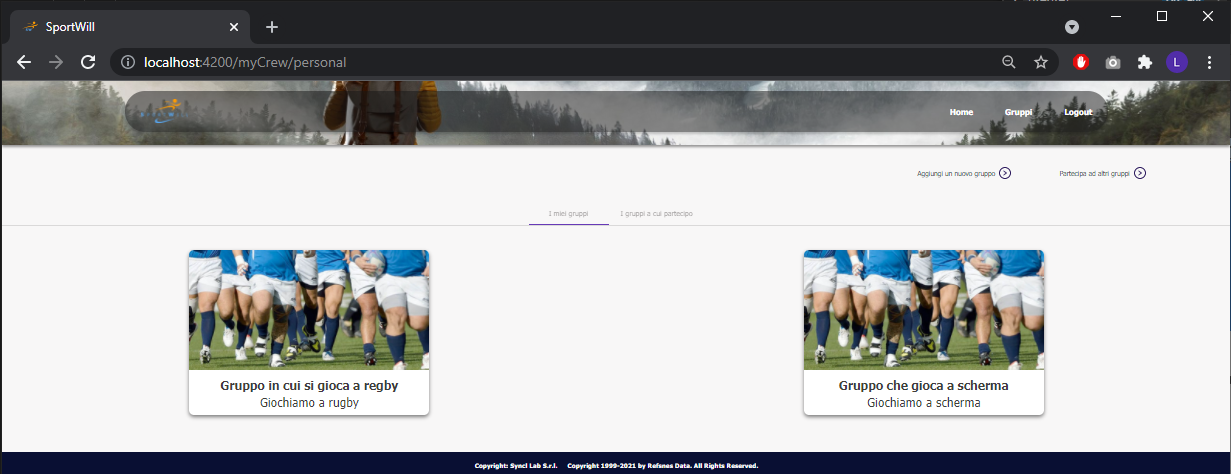
\includegraphics[scale=0.6]{sito/i-miei-gruppi.png}
    \caption{Pagina dei gruppi creati o a cui partecipa un utente}
\end{figure}
\mysubparagraph{Componenti utilizzati}
\begin{itemize}
    \item \hyperref[par:Crewpage]{Crewpage}
          % \item \hyperref[par:CrewCard]{CrewCard}
\end{itemize}
% \mysubparagraph{Servizi}
% \begin{itemize}
%     \item \hyperref[par:GruppiService]{GruppiService}
% \end{itemize}

\myparagraph{Gruppi}
\label{par:Gruppi}
Questa pagina permette ad un utente autenticato di visualizzare i gruppi a cui
può partecipare, senza visualizzare i gruppi a cui già partecipa.
\begin{figure}[H]
    \centering
    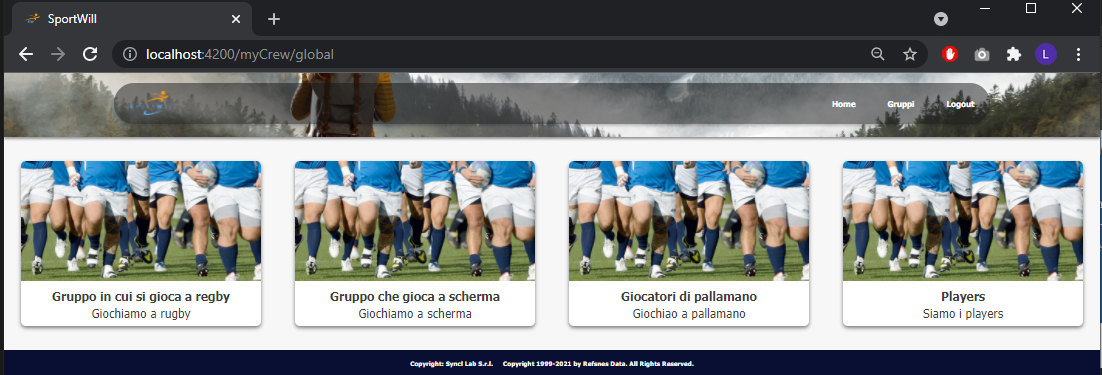
\includegraphics[scale=0.6]{sito/gruppi-pagina.png}
    \caption{Pagina dei gruppi}
\end{figure}
\mysubparagraph{Componenti utilizzati}
\begin{itemize}
    \item \hyperref[par:Crewpage]{Crewpage}
          % \item \hyperref[par:CrewCard]{CrewCard}
\end{itemize}
% \mysubparagraph{Servizi}
% \begin{itemize}
%     \item \hyperref[par:GruppiService]{GruppiService}
% \end{itemize}

\myparagraph{Crea nuovo gruppo}
\label{par:Crea nuovo gruppo}

Questa pagina permette ad un utente autenticato di creare un nuovo gruppo.
\begin{figure}[H]
    \centerline{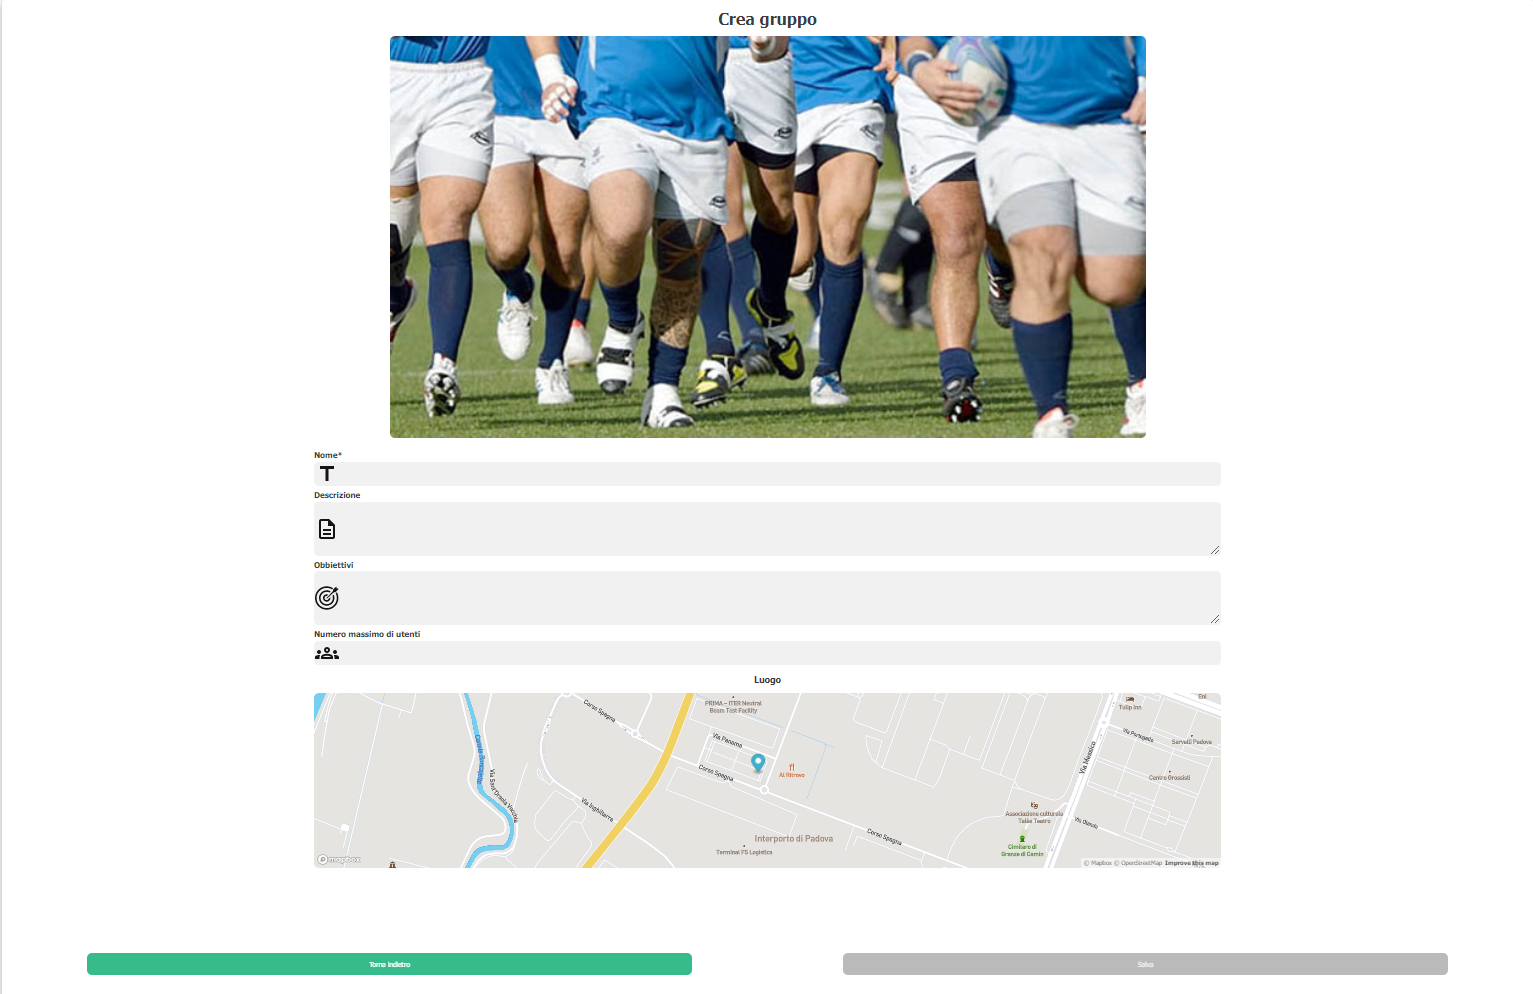
\includegraphics[scale=0.25]{sito/crea-gruppo.png}}
    \caption{Pagina di creazione di un gruppo}
\end{figure}
\mysubparagraph{Componenti utilizzati}
\begin{itemize}
    \item \hyperref[par:CrewDetail]{CrewDetail}
\end{itemize}
% \mysubparagraph{Servizi}
% \begin{itemize}
%     \item \hyperref[par:GruppiService]{GruppiService}
% \end{itemize}

\myparagraph{Modifica un gruppo}
Questa pagina permette ad un utente autenticato di modificare i dettagli di un
gruppo.
\begin{figure}[H]
    \centerline{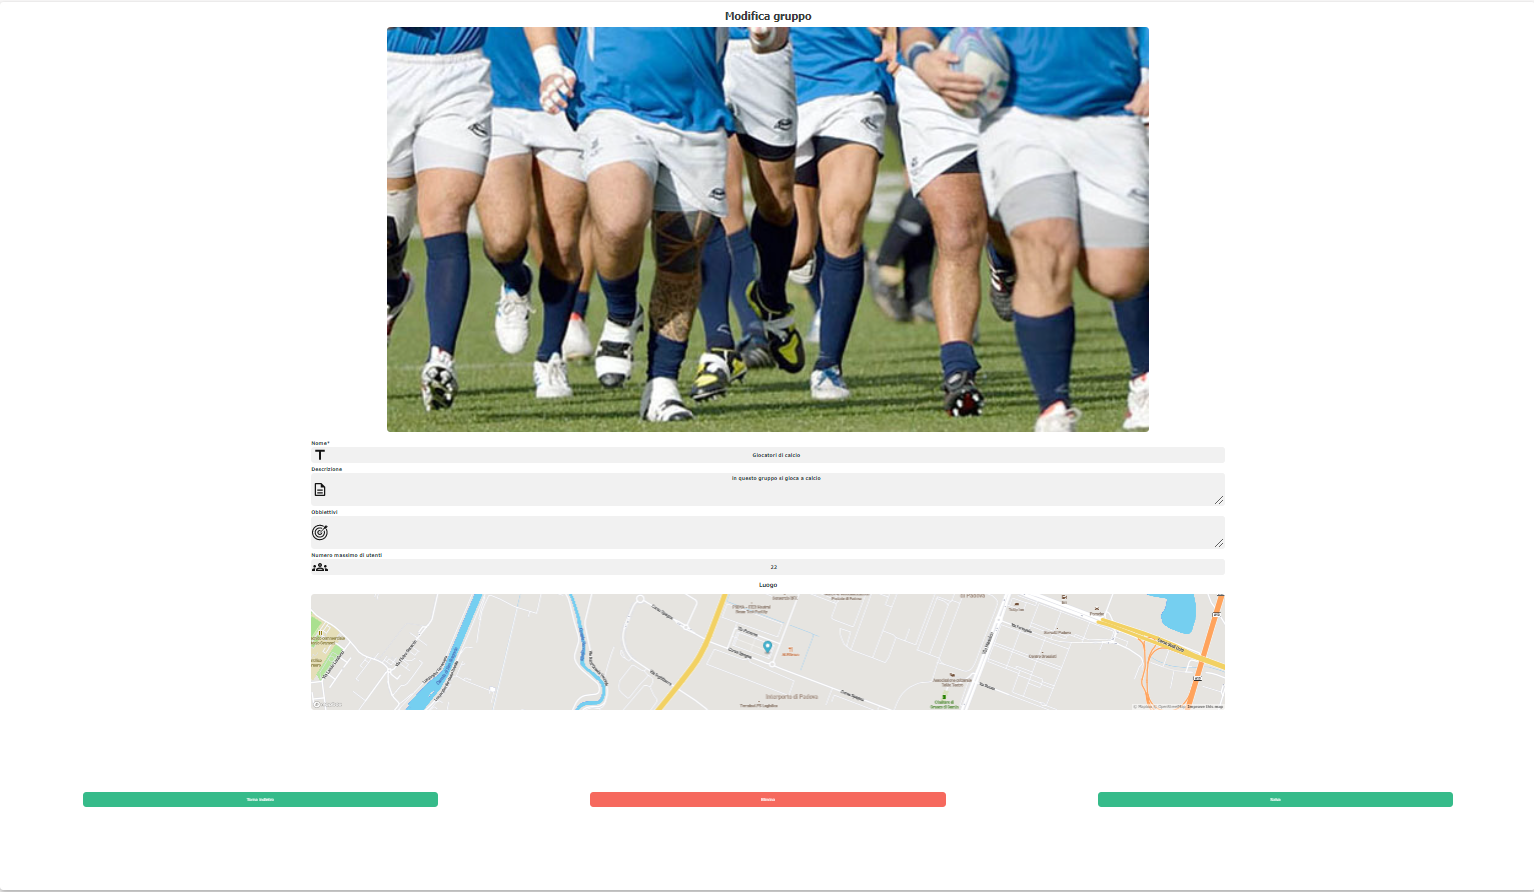
\includegraphics[scale=0.25]{sito/modifica-gruppo.png}}
    \caption{Pagina di modifica di un gruppo}
\end{figure}
\mysubparagraph{Componenti utilizzati}
\begin{itemize}
    \item \hyperref[par:CrewEditable]{CrewEditable}
\end{itemize}
% \mysubparagraph{Servizi}
% \begin{itemize}
%     \item \hyperref[par:GruppiService]{GruppiService}
% \end{itemize}

\myparagraph{Visualizza dettagli di un gruppo}
Questa pagina permette ad un utente autenticato di visualizzare i dettagli di
un gruppo.
\begin{figure}[H]
    \centerline{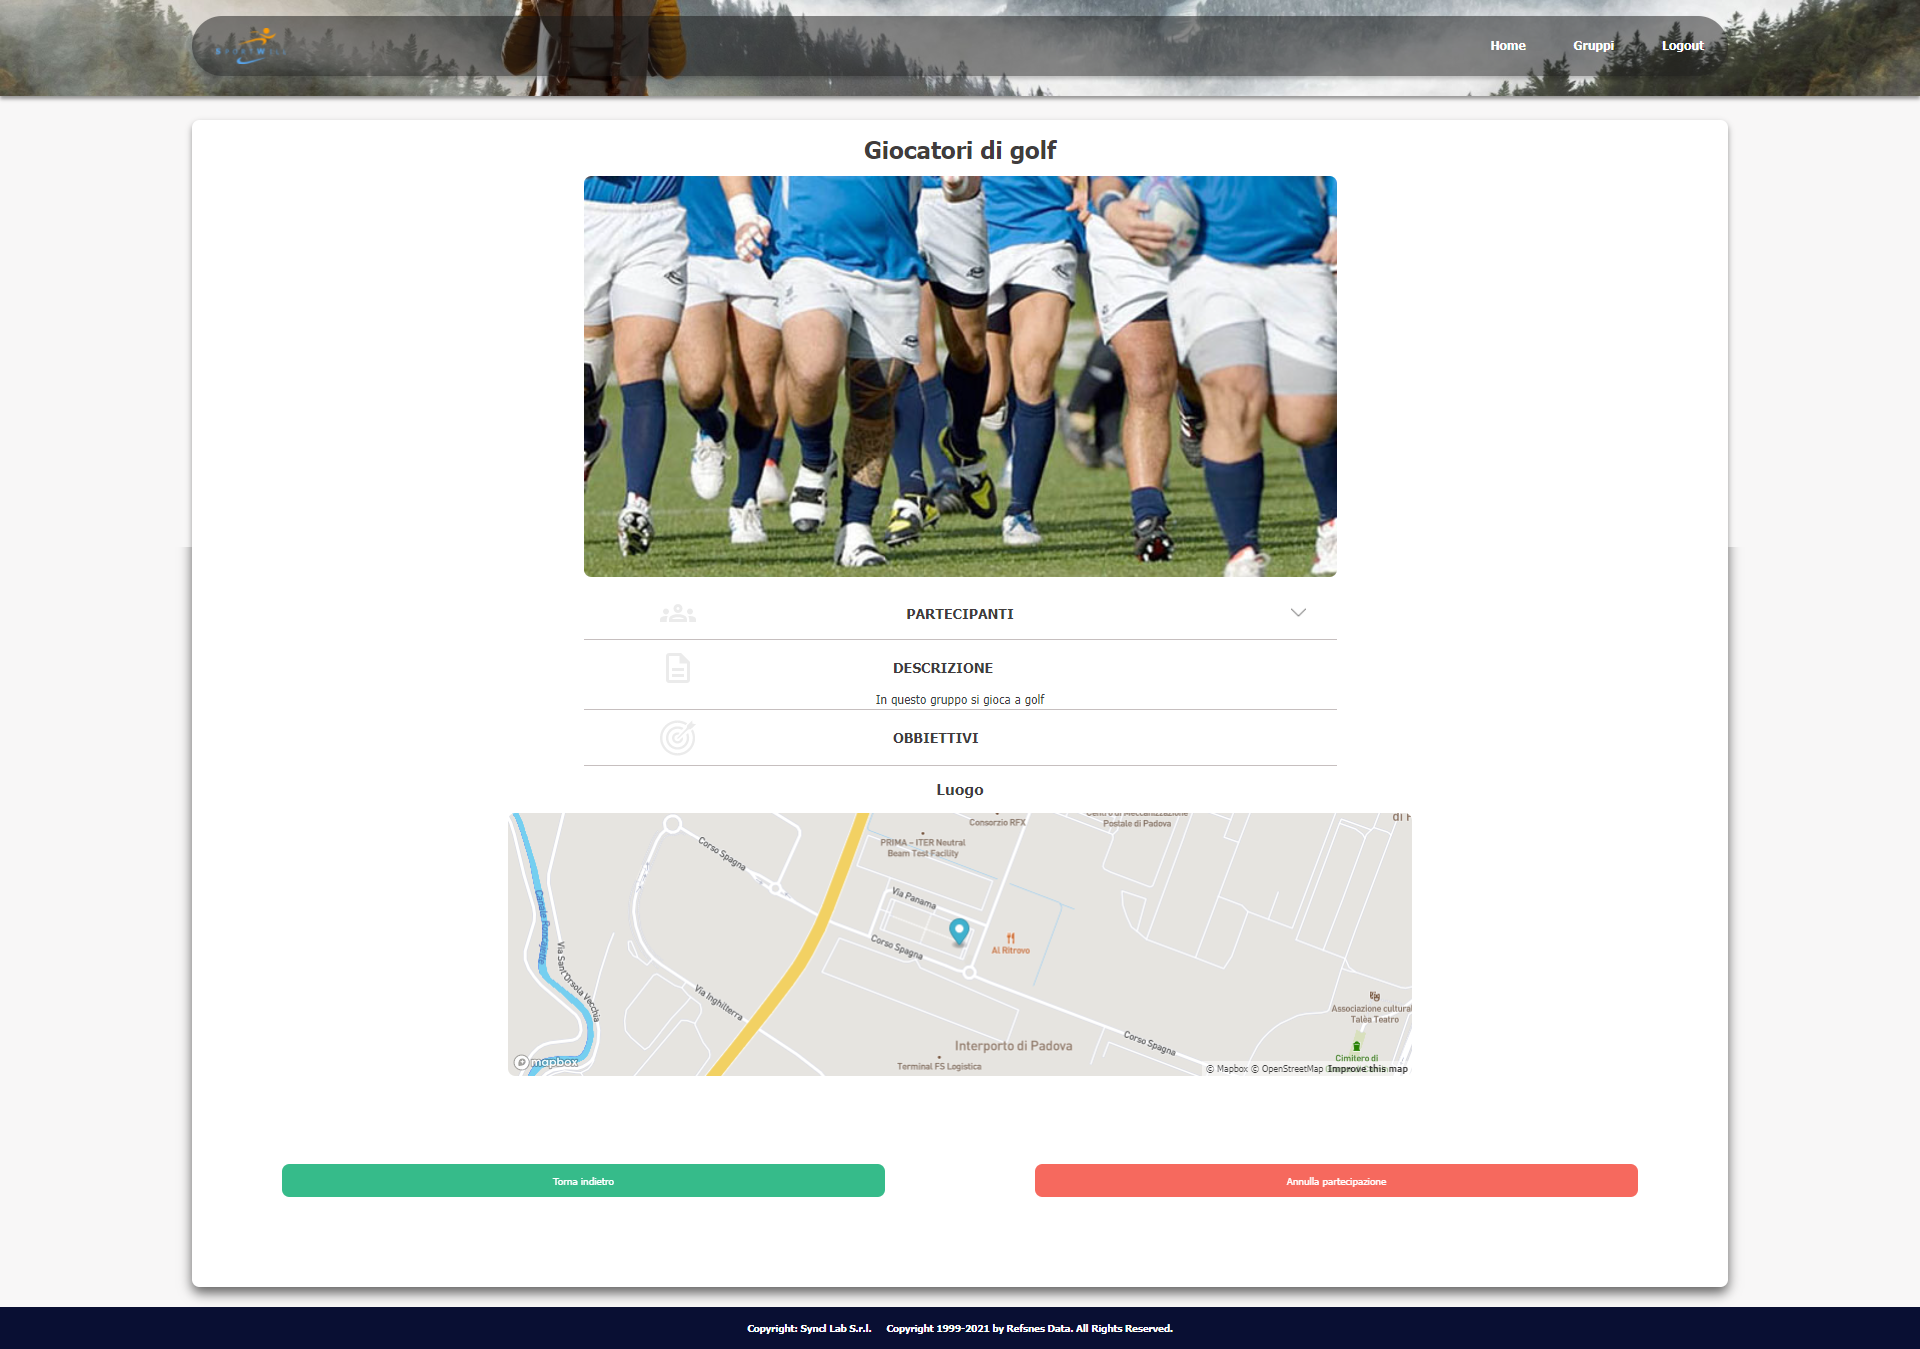
\includegraphics[scale=0.25]{sito/dettagli-gruppo.png}}
    \caption{Pagina di visualizzazione dei dettagli di un gruppo}
\end{figure}
\mysubparagraph{Componenti utilizzati}
\begin{itemize}
    \item \hyperref[par:CrewDetail]{CrewDetail}
\end{itemize}
% \mysubparagraph{Servizi}
% \begin{itemize}
%     \item \hyperref[par:GruppiService]{GruppiService}
% \end{itemize}

\subsubsection{Componenti}
\myparagraph{HomepageComponent}
\label{par:HomepageComponent}
Questo componente è composto da una lista di \nameref{par:WillCard}, ed ha le
seguenti funzionalità:
\begin{itemize}
    \item visualizzare le \gls{will} visibili a tutti gli utenti (anche quelli
          non autenticati);
    \item visualizzare le \gls{will} dell'utente nel caso sia autenticato;
    \item visualizzare le \gls{will} dei gruppi a cui appartiene l'utente nel
          caso sia autenticato.
\end{itemize}

\begin{figure}[H]

    \centerline{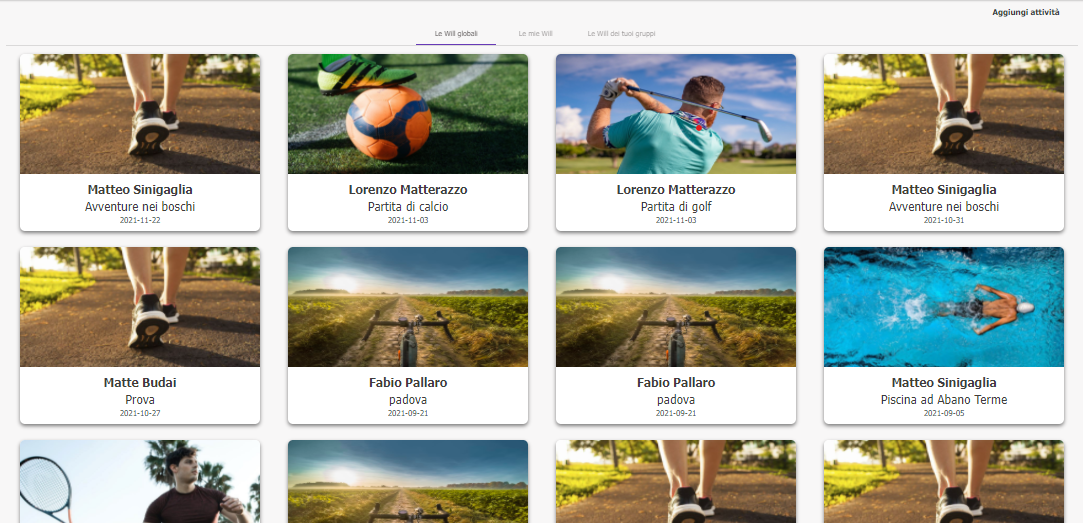
\includegraphics[scale=0.8]{sito/component/homepage-component.png}}
    \caption{Componente \texttt{Homepage} di un utente autenticato}
\end{figure}

\begin{figure}[H]

    \centerline{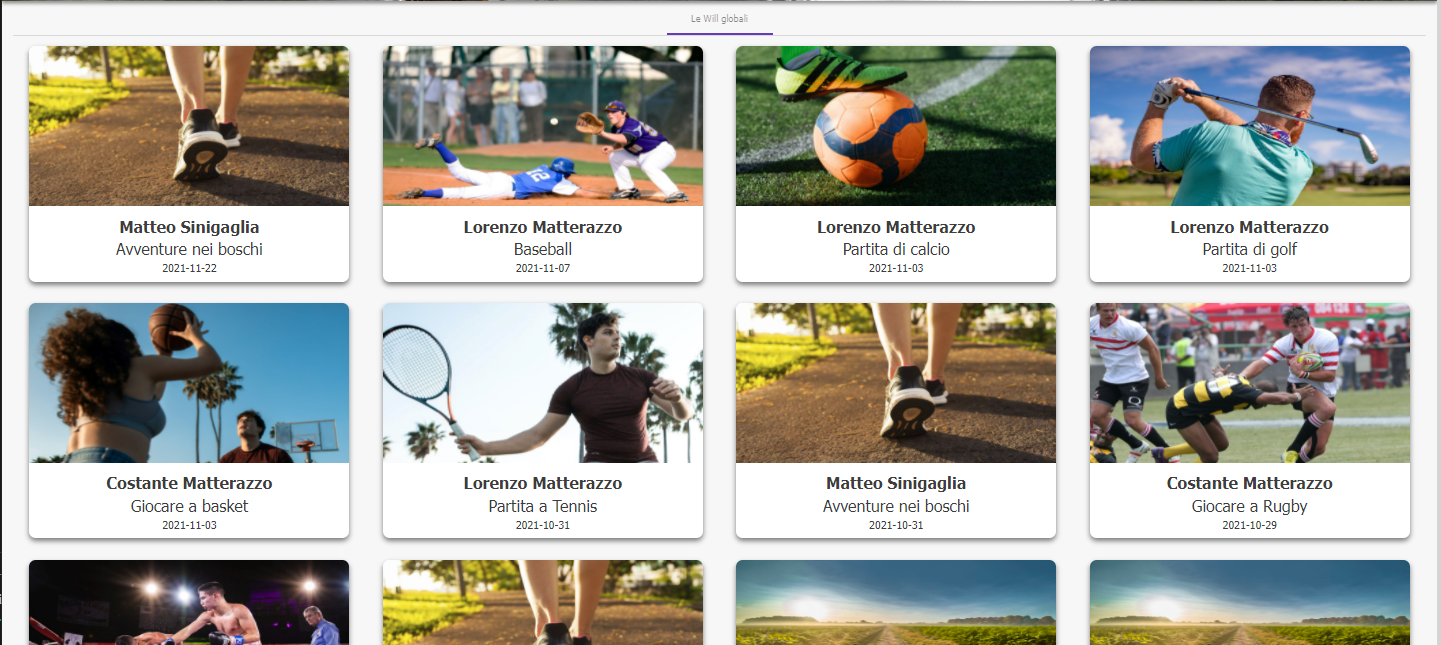
\includegraphics[scale=0.6]{sito/component/homepage-non-autenticato.png}}
    \caption{Componente \texttt{Homepage} di un utente non autenticato}
\end{figure}

% \myparagraph{Servizi}
% \begin{itemize}
%     \item \nameref{par:WillDataService}
%     \item \nameref{par:GruppiService}
% \end{itemize}

\myparagraph{Metodi}
\begin{itemize}
    \item \class{ngOnInit}: all'inizializzazione del componente viene
          controllato, mediante il servizio \texttt{AuthenticationService}(non
          implementato da me), se l'utente è autenticato, in modo da valutare
          se
          visualizzare anche le schermate \enquote*{le mie Will} e \enquote*{le
              Will dei
              tuoi gruppi} o meno;
    \item \class{getDataWithGlobalVisibility}: ottiene le \gls{will} con
          visibilità globale;
    \item \class{getDataPersonal}: ottiene le \gls{will} create dall'utente;
    \item \class{getDataCrew}: ottiene le \gls{will} dei gruppi a cui
          appartiene l'utente;
    \item \class{orderCards}: ordina le \gls{will} in base alla data d'uscita.
\end{itemize}

\myparagraph{WillCard}
\label{par:WillCard}
Questo componente, implementato da un collega, permette di visualizzare
l'anteprima di una \gls{will}, in particolare:
\begin{itemize}
    \item Il nome dell'organizzatore;
    \item lo sport relativo all'uscita;
    \item la data d'uscita.
\end{itemize}

\begin{figure}[H]
    \centering
    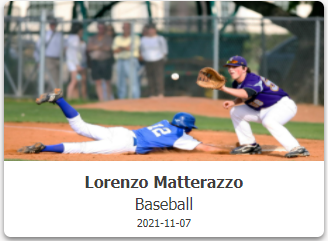
\includegraphics[scale=1]{sito/component/card-component.png}
    \caption{Componente \texttt{WillCard}}
\end{figure}

\myparagraph{CrewCard}
\label{par:CrewCard}
Questo componente permette di visualizzare l'anteprima di una gruppo, in
particolare:
\begin{itemize}
    \item il nome del gruppo;
    \item la descrizione.
\end{itemize}

\begin{figure}[H]
    \centering
    
\includegraphics[scale=1]{sito/component/crew-component.png}
    \caption{Componente \texttt{CrewCard}}
\end{figure}

% \myparagraph{Servizi}
% \begin{itemize}
%     \item \nameref{par:GruppiService}
% \end{itemize}
\myparagraph{Input}
\begin{itemize}
    \item \class{crew}: gruppo da visualizzare.
\end{itemize}

\myparagraph{Metodi}
\begin{itemize}
    \item \class{navigate}: permette di navigare alla pagina di visualizzazione
          dei dettagli del gruppo. Se il gruppo cliccato è stato creato
          dall'utente
          allora viene visualizzato il \textit{component}
          \nameref{par:CrewEditable},
          altrimenti \nameref{par:CrewDetail}.
\end{itemize}

\myparagraph{Crewpage}
\label{par:Crewpage}
Questo componente è composto da una lista di \nameref{par:CrewCard}, e permette
di visualizzare le maschere dei \hyperref[par:Gruppi dell'utente]{gruppi
    dell'utente} e \hyperref[par:Gruppi]{gruppi a cui è possibile partecipare}.

\begin{figure}[H]
    \centering
    
\includegraphics[scale=0.6]{sito/component/gruppi-globali-component.png}
    \caption{Componente \texttt{Crewpage} che visualizza i gruppi in cui
        partecipare}
\end{figure}

\begin{figure}[H]
    \centering
    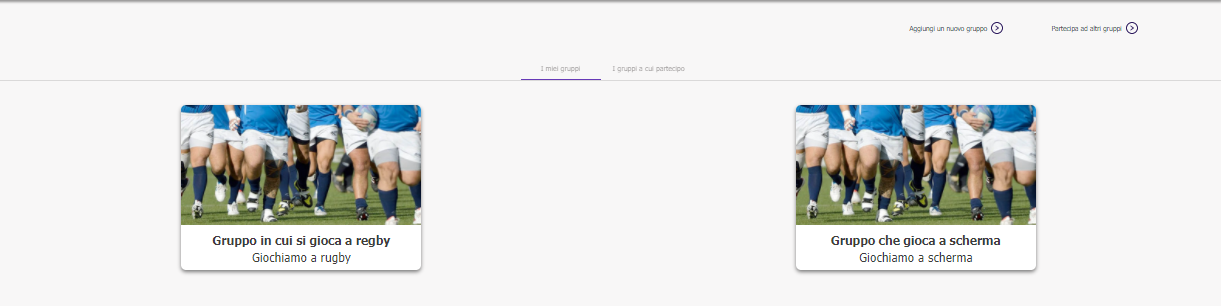
\includegraphics[scale=0.6]{sito/component/i-miei-gruppi-component.png}
    \caption{Componente \texttt{Crewpage} che visualizza la pagina di gestione
        dei gruppi dell'utente}
\end{figure}

% \myparagraph{Servizi}
% \begin{itemize}
%     \item \nameref{par:GruppiService}
% \end{itemize}

\myparagraph{Metodi}
\begin{itemize}
    \item \class{ngOnInit}: all'inizializzazione del componente viene valutato
          se visualizzare la schermata \nameref{par:Gruppi dell'utente} o
          \nameref{par:Gruppi};
    \item \class{getGlobalCrew}: ottiene i gruppi a cui non partecipa un
          utente;
    \item \class{getUserCrew}:	ottiene i gruppi create e a cui partecipa un
          utente;
    \item \class{navigateToNewCrew}: permette di navigare alla pagina di
          \hyperref[par:Crea nuovo gruppo]{creazione di un nuovo gruppo};
    \item \class{navigateToGlobalCrew}: permette di navigare alla pagina di
          visualizzazione dei \hyperref[par:Gruppi]{gruppi}.
\end{itemize}

\myparagraph{CrewDetail}
\label{par:CrewDetail}
Questo componente permette di visualizzare i dettagli di un gruppo.
\begin{figure}[H]
    \centering
    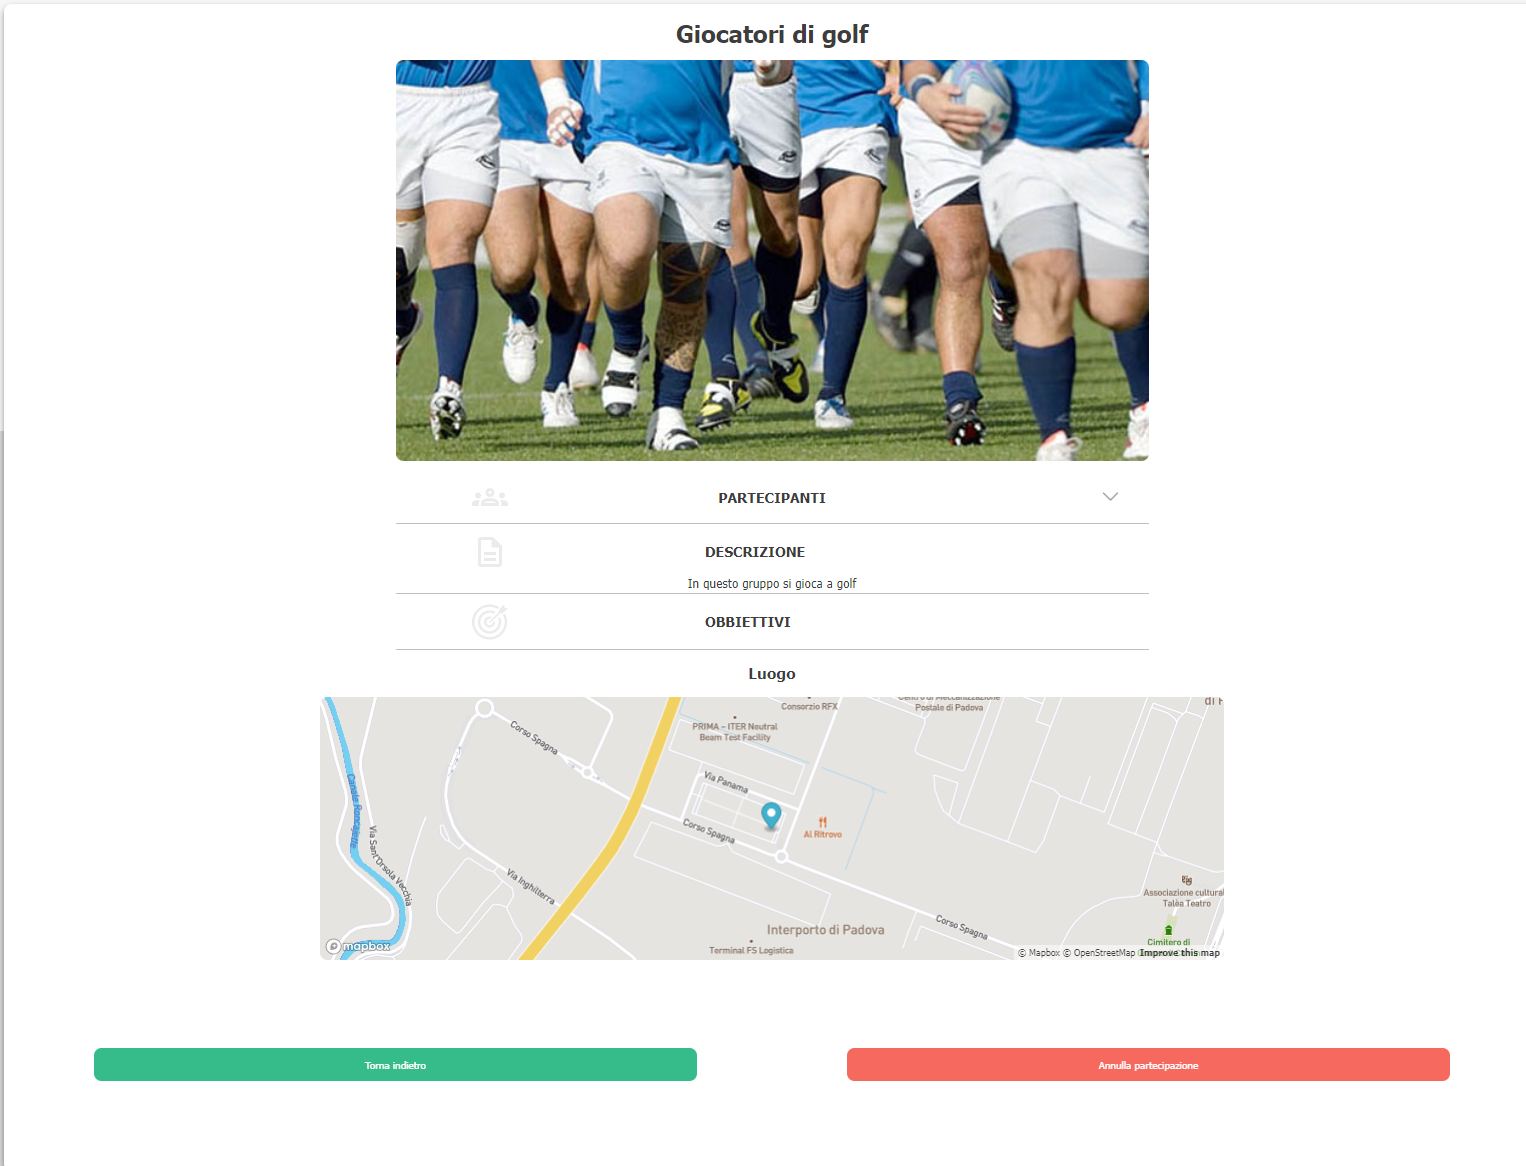
\includegraphics[scale=0.3]{sito/component/dettagli-gruppo-component.png}
    \caption{Componente che permette di visualizzare i dettagli di un gruppo}
\end{figure}
\myparagraph{Componenti}
\begin{itemize}
    \item \nameref{par:MapComponent}
\end{itemize}

% \myparagraph{Servizi}
% \begin{itemize}
%     \item \nameref{par:GruppiService}
% \end{itemize}

\myparagraph{Metodi}
\begin{itemize}
    \item \class{getParticipants}: ottiene gli utenti che partecipano al
          gruppo;
    \item \class{addParticipant}: aggiunge l'utente ad un gruppo;
    \item \class{removeParticipant}: rimuove l'utente da un gruppo;
    \item \class{getCrew}: ottiene i dettagli di un gruppo.
\end{itemize}

\myparagraph{CrewEditable}
\label{par:CrewEditable}

Questo componente permette di modificare i dettagli di un gruppo.
\begin{figure}[H]

    \centerline{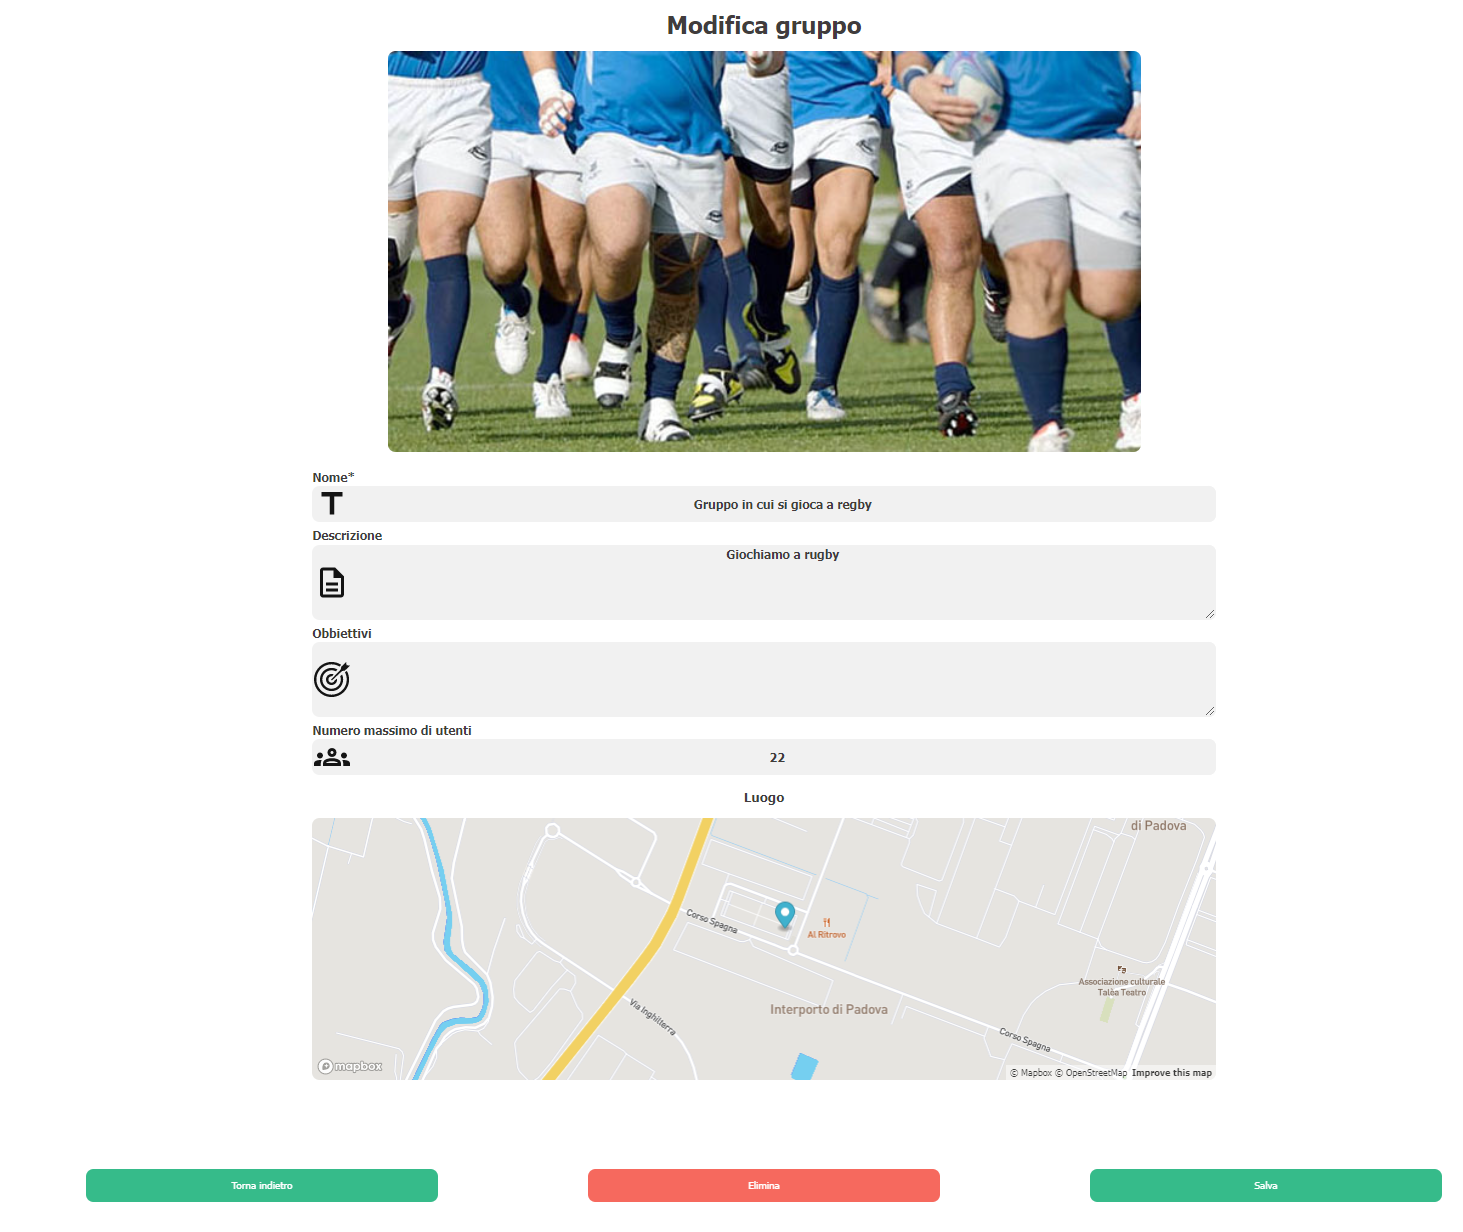
\includegraphics[scale=0.4]{sito/component/modifica-gruppo-component.png}}

    \caption{Componente \texttt{CrewEditable}}
\end{figure}
\myparagraph{Componenti}
\begin{itemize}
    \item \nameref{par:MapComponent}
    \item \nameref{par:Dialog}
\end{itemize}

% \myparagraph{Servizi}
% \begin{itemize}
%     \item \nameref{par:GruppiService}
% \end{itemize}

\myparagraph{Metodi}
\begin{itemize}
    \item \class{getCrew}: ottiene i dettagli di un gruppo;
    \item \class{deleteCrew}: elimina il gruppo in questione. È richiesta la
          conferma dell'operazione attraverso il \hyperref[par:Dialog]{dialog}
          per
          confermare l'eliminazione;
    \item \class{saveCrew}: salva le modifiche effettuate ai dettagli del
          gruppo. È richiesta la conferma dell'operazione attraverso il
          \hyperref[par:Dialog]{dialog} per confermare la modifica;
\end{itemize}

\myparagraph{DialogComponent}
\label{par:Dialog}
Questo componente serve per confermare le operazioni effettuano delle modifiche
all'applicativo.

\begin{figure}[H]
    \centering
    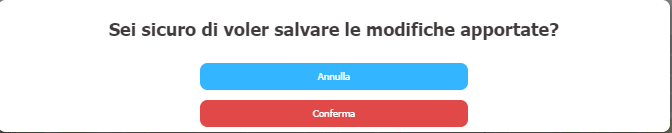
\includegraphics[scale=1]{sito/component/dialog-component.png}
    \caption{Componente \texttt{DialogComponent}}
\end{figure}

\myparagraph{Input}
\begin{itemize}
    \item \class{message}: testo del messaggio da visualizzare.
\end{itemize}

\myparagraph{Output}
\begin{itemize}
    \item \class{clicked}: segnale emesso quando viene cliccata un'opzione. Il
          segnale emesso è di tipo \textit{booleano} ed indica se l'azione è
          stata
          confermata o meno.
\end{itemize}

\myparagraph{Metodi}
\begin{itemize}
    \item \class{buttonClicked}: emette l'evento \texttt{clicked}.
\end{itemize}

\myparagraph{MapComponent}
\label{par:MapComponent}
Questo componente permette di visualizzare una mappa in cui viene segnato con
un \textit{marker} nelle coordinate specifiche nei campi \texttt{latitudine} e
\texttt{longitudine}.
\begin{figure}[H]
    \centerline{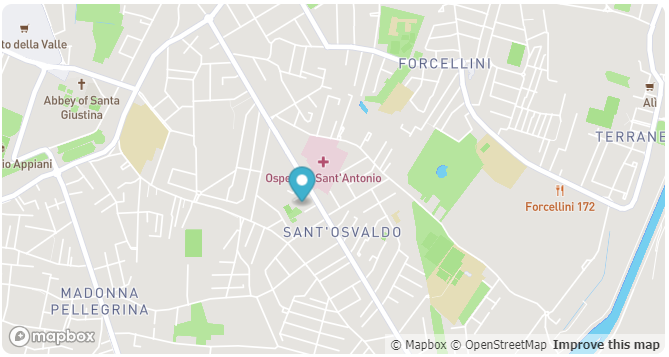
\includegraphics[scale=0.55]{sito/component/map-component.png}}

    \caption{Componente \texttt{MapComponent}}
\end{figure}

\myparagraph{Input}
\begin{itemize}
    \item \class{latitudine};
    \item \class{longitudine};
    \item \class{editable}: specifica se è possibile modificare il
          \textit{marker} nella mappa.
\end{itemize}

\myparagraph{Output}
\begin{itemize}
    \item \class{latitudineChanged}: segnale emesso quando viene spostato il
          \textit{marker}. Emette il nuovo valore per la latitudine;
    \item \class{longitudineChanged}: segnale emesso quando viene spostato il
          \textit{marker}. Emette il nuovo valore per la longitudine.
\end{itemize}

\myparagraph{Metodi}
\begin{itemize}
    \item \class{ngOnInit}: all'inizializzazione del componente viene valutato
          se la mappa sia modificabile o no; nel caso lo fosse viene effettuato
          un
          \textit{binding} fra il \textit{click} sulla mappa e la funzione
          \texttt{modify\_marker};
    \item \class{modify\_marker}: modifica le coordinate da visualizzare sulla
          mappa in caso questa venga modificata. Emette inoltre i segnali
          \texttt{latitudineChanged} e \texttt{longitudineChanged}.
\end{itemize}

\subsection{Servizi}
% Descrizione del servizio
% Metodi
\myparagraph{GruppiService}
\label{par:GruppiService}
Servizio che si occupa di effettuare chiamate HTTP al \textit{back end} per
richiedere, gestire e modificare i gruppi.

\mysubparagraph{Metodi}
\begin{itemize}
    \item \class{getCrews}: ottiene la lista di tutti i gruppi;
    \item \class{addCrew}: inserisce un nuovo gruppo alla lista dei gruppi;
    \item \class{getInfoCrew}: ottiene le informazioni di un gruppo specifico;
    \item \class{modifyCrew}: modifica i dettagli di un gruppo;
    \item \class{getAllUsciteofCrew}: ottiene tutte le uscite di un gruppo;
    \item \class{getUsersOfCrew}: ottiene gli utenti di un gruppo;
    \item \class{deleteCrew}: elimina un gruppo;
    \item \class{getCrewsOfUser}: ottiene tutti i gruppi a cui appartiene un
          utente;
    \item \class{addUserToCrew}: aggiunge un utente ad un gruppo;
    \item \class{removeUserFromCrew}: rimuove un utente da un gruppo.
\end{itemize}